\documentclass[conference]{IEEEtran}
\usepackage{times}

% numbers option provides compact numerical references in the text. 
\usepackage[numbers]{natbib}
\usepackage{multicol}
\usepackage[bookmarks=true]{hyperref}
%\usepackage[inline]{enumitem}

\pdfinfo{
   /Author (author)
   /Title  (title)
   /CreationDate (D:20101201120000)
   /Subject (Robots)
   /Keywords (Robots)
}

\usepackage{microtype}
\usepackage{amsmath,amssymb}
\usepackage{paralist}
\usepackage{mdframed}
\usepackage{xcolor}
\usepackage{tikz}
\usepackage{amsthm}
\usepackage{amssymb}
\usepackage{nicefrac}
\usepackage{amsthm}
\usepackage{colonequals}
\newtheorem{theorem}{Theorem}
\newtheorem{proposition}{Proposition}
\theoremstyle{remark}
\newtheorem{remark}{Remark}
\newtheorem{example}{Example}
\newtheorem{definition}{Definition}
\usepackage{import}
\usepackage{pgf}


\usepackage{todonotes}
\usepackage{pgfplots}
\usepackage{algorithm, algorithmicx}
\usepackage[noend]{algpseudocode}

\usepgfplotslibrary{fillbetween}
\usetikzlibrary{patterns,arrows,backgrounds,calc,shapes,shadows,decorations.pathmorphing,decorations.pathreplacing,automata,shapes.multipart,positioning,shapes.geometric,fit,circuits,trees,shapes.gates.logic.US,fit,decorations.markings}

\tikzset{sstate/.style={circle, draw=black, inner sep=1pt,minimum height=6mm}}
\tikzset{astate/.style={diamond, draw=black, inner sep=1pt}}
\tikzset{tstate/.style={rectangle, draw=black, inner sep=1pt, minimum height=5mm}}
\tikzset{actnode/.style={fill=black, inner sep=1pt}}
\tikzset{elab/.style={auto,font={\fontsize{9pt}{12}\selectfont}}}

\tikzset{cross/.style={cross out, draw=black, minimum size=2*(#1-\pgflinewidth), inner sep=0pt, outer sep=0pt},
%default radius will be 1pt. 
cross/.default={1pt}}

\makeatletter
\let\MYcaption\@makecaption
\makeatother

\usepackage[font=footnotesize]{subcaption}

\makeatletter
\let\@makecaption\MYcaption
\makeatother

\newcommand{\Nat}{\mathbb{N}}
\newcommand{\NN}{\mathbb{N}}
\newcommand{\mc}{\mathcal{D}}
\newcommand{\sg}{\mathcal{G}}
\renewcommand{\path}{\xi}
\newcommand{\eventually}[1]{\lozenge^{\leq #1}}
\newcommand{\sched}{\sigma}
\newcommand{\Sched}{\Sigma}
\newcommand{\pol}{\sched}
\newcommand{\Distr}{\ensuremath{\textsl{Distr}}}
\newcommand{\act}{\alpha}
\newcommand{\altact}{\beta}
\newcommand{\Act}{A}
\newcommand{\scp}{p}
\newcommand{\scthreshold}{\mathbf{p}}
\newcommand{\scregret}{\epsilon_p}
\newcommand{\target}{s_{\top}} 
\newcommand{\sink}{s_{\bot}}
\newcommand{\rndp}{h}
\newcommand{\randomness}{\mathbf{h}}
\newcommand{\randomnessReget}{\epsilon_h}
\newcommand{\last}[1]{\mathsf{last}({#1})}
\newcommand{\pOneSched}{{\sigma_\pOne}}
\newcommand{\pOneSchedPrime}{{\sigma'_\pOne}}
\newcommand{\pOneSchedPrimePrime}{{\sigma''_\pOne}}
\newcommand{\POneScheds}{\Sigma_\pOne}
\newcommand{\PTwoScheds}{\Sigma_\pTwo}
\newcommand{\pTwoSched}{{\sigma_\pTwo}}
\newcommand{\pTwoSchedWorstH}{{\sigma_\pTwo^H}}
\newcommand{\rat}{\lambda}
\newcommand{\pOne}{\mathsf{ego}}
\newcommand{\pTwo}{\mathsf{env}}
\newcommand{\player}{\mathsf{i}}
\newcommand{\horizon}{\tau}
\newcommand{\solutions}{\mathbb{S}}
\newcommand{\EnAct}{\Act}
\newcommand{\solfuncp}{f_\mathbb{S}}
\newcommand{\scopt}{\scp^{*}}
\newcommand{\rndopt}{\rndp^{*}}
\newcommand{\pareto}[1]{\mathcal{F}_{#1}}
\newcommand{\smoothmax}{\operatorname*{\mathrm{smax}}}
\newcommand{\indicator}[1]{[#1]}
\newcommand{\Succ}{\mathsf{Succ}}

\newcommand{\supp}{\mathsf{support}}
\newcommand{\ppthreshold}{\mathbf{d}}

\newcommand{\scmin}{\scp^{-}}
\newcommand{\rndmin}{\rndp^{-}}
% \newcommand{\pathslbl}{\Xi}
\newcommand{\pathslbl}{\mathsf{Paths}}
\newcommand{\Paths}[2][]{\pathslbl^{#2}_{#1}}
\newcommand{\POnePaths}[2][]{{[\pathslbl^{#2}_{#1}]_\pOne}}
\newcommand{\PTwoPaths}[2][]{{[\pathslbl^{#2}_{#1}]_\pTwo}}
\newcommand{\PlayerPaths}[2][]{{[\pathslbl^{#2}_{#1}]}_{\player}}
\newcommand{\unrolled}[2]{\textsf{Tree}(#1,#2)}
\newcommand{\induced}[2]{#1[#2]}
\newcommand{\causalprob}[2]{\Pr(#1\mid\mid#2)}
\newcommand{\E}{\operatorname*{\mathbb{E}}}
\newcommand{\expOver}[2]{\mathbb{E}_{#1}[#2]}
\newcommand{\soft}{\varphi}
\newcommand{\hard}{\psi}
\newcommand{\rv}[1]{{\mathcal{#1}}}  % Random Variable
\newcommand{\droneEnv}{{D_{\text{new}}}}
\newcommand{\droneEgo}{{D_{\text{test}}}}


\newcommand{\eqdef}{\mathrel{\stackrel{\makebox[0pt]{\mbox{\normalfont\tiny def}}}{=}}}
\newcommand{\mypara}[1]{\noindent{\bf #1.}}
\newcommand{\propref}[1]{{Prop.~\ref{prop:#1}}}
\newcommand{\secref}[1]{{Sec.~\ref{sec:#1}}}

\newcommand{\UPDATE}{{\mathsf{update}}}

\setlength\marginparwidth{110pt}
\newcommand{\colorpar}[3]{\colorbox{#1}{\parbox{#2}{#3}}}
\newcommand{\marginremark}[3]{\marginpar{\colorpar{#2}{\linewidth}{\color{#1}#3}}}
\newcommand{\commentside}[2]{\marginpar{\color{#1}\tiny#2}}
\newcommand{\TODO}[1]{\commentside{teal}{\textsc{Todo:} #1}}
\newcommand{\REMARK}[1]{\commentside{teal}{\textsc{Remark:} #1}}\newcommand{\sj}[1]{\marginremark{black}{red!10!white}{\scriptsize{[SJ]~ #1}}}
\newcommand{\mvc}[1]{\marginremark{black}{gray!10!white}{\scriptsize{[MVC]~ #1}}}

\newtheorem{lemma}{Lemma}
\newtheorem{corollary}{Corollary}

%\institute{University of California, Berkeley, CA, USA}


\begin{document}

% paper title
\title{Entropy-Guided Control Improvisation}

% You will get a Paper-ID when submitting a pdf file to the conference system
% \author{Author Names Omitted for Anonymous Review. Paper-ID 177}


\author{
  \authorblockN{
    Marcell Vazquez-Chanlatte\authorrefmark{1},
    Sebastian Junges\authorrefmark{1},
    Daniel J. Fremont\authorrefmark{2},
    Sanjit A. Seshia\authorrefmark{1}
  }
  \authorblockA{
    University of California, \{Berkeley\authorrefmark{1}, Santa Cruz\authorrefmark{2}\}
  }
}

% avoiding spaces at the end of the author lines is not a problem with
% conference papers because we don't use \thanks or \IEEEmembership


% for over three affiliations, or if they all won't fit within the width
% of the page, use this alternative format:
% 
%\author{\authorblockN{Michael Shell\authorrefmark{1},
%Homer Simpson\authorrefmark{2},
%James Kirk\authorrefmark{3}, 
%Montgomery Scott\authorrefmark{3} and
%Eldon Tyrell\authorrefmark{4}}
%\authorblockA{\authorrefmark{1}School of Electrical and Computer Engineering\\
%Georgia Institute of Technology,
%Atlanta, Georgia 30332--0250\\ Email: mshell@ece.gatech.edu}
%\authorblockA{\authorrefmark{2}Twentieth Century Fox, Springfield, USA\\
%Email: homer@thesimpsons.com}
%\authorblockA{\authorrefmark{3}Starfleet Academy, San Francisco, California 96678-2391\\
%Telephone: (800) 555--1212, Fax: (888) 555--1212}
%\authorblockA{\authorrefmark{4}Tyrell Inc., 123 Replicant Street, Los Angeles, California 90210--4321}}


\maketitle

\begin{abstract}
  % Sentence 1: State the problem
  High level declarative constraints provide a powerful (and popular)
  way to define and construct control policies; however, most
  synthesis algorithms do not support specifying the degree of
  randomness (unpredictability) of the resulting controller.
  % Sentence 2: State the consequences
  In many contexts, e.g., patrolling, testing, behavior prediction,
  and planning on idealized models, predictable or biased controllers
  are undesirable.
  % Sentence 3: State your solution
  To address these concerns, we introduce the \emph{Entropic Reactive
    Control Improvisation} (ERCI) framework and algorithm which
  supports synthesizing control policies for stochastic games that are
  declaratively specified by (i) a \emph{hard constraint} specifying
  what must occur (ii) a \emph{soft constraint} specifying what
  typically occurs, and (iii) a \emph{randomization constraint}
  specifying the unpredictability and variety of the
  controller, as quantified using causal entropy.
  % Sentence 4: State the consequences of the solution
  This framework, which extends the state-of-the-art by supporting
  arbitrary combinations of adversarial and probabilistic uncertainty
  in the environment, enables a flexible modeling formalism which
  we argue, theoretically and empirically, remains tractable.
\end{abstract}

\IEEEpeerreviewmaketitle

%\maketitle\sj{Daniel?}
%\begin{abstract}
%	Efficacious controller synthesis is a key ingredient in the design and analysis of complex systems. We study the design of controllers that have a high entropy, that is, whose behavior or nature is surprising. The synthesis of such controllers is key in domains like testing and security. 
%	In particular, our paper studies control improvisation and compares them with randomly sampling adequate policies. The only difference in obtained policies is in their notion of entropy, but the problems are significantly different.  We illustrate and contrast their merits and limitations. Furthermore, we provide algorithms that solve both control improvisation problems. Prominently, we solve the control improvisation problem for Markov decision processes by relating it to recent results from inference from demonstrations, and then extend this approach to stochastic games. We present a prototypical implementation that efficiently solves controller synthesis problems from the security and testing domain. 
%\end{abstract}
\section{Introduction}
% Declarative Constraints ar neat idea.
The use of declarative specifications, e.g. in the form of temporal logic formulas, has become a popular way to construct high-level robot controllers~\cite{DBLP:conf/iros/HorowitzWM14, DBLP:conf/rss/WongEK14, DBLP:conf/iros/HeLKV17, DBLP:conf/icra/FuATP16, DBLP:conf/icra/HeWKV19, DBLP:journals/arobots/MoarrefK20, DBLP:conf/icra/KantarosM0P20}.
% Synthesis closes the gap.
Given a user provided specification, \emph{synthesis} algorithms aim
to automatically create a control policy that ensures that the
specification is met, or explain why such a policy does not
exist. Together, synthesis and declarative specifications facilitate
quickly and intuitively solving a wide variety of control tasks.  For
example, consider a delivery drone operating in a workspace. One may
specify the drone should ``within 10 minutes, visit four locations (in any
order) \emph{and} avoid crashing.''. A synthesis tool may then create a
finite state controller which guarantees this specification is met,
under a particular world model.
% Declarative Synthesis need not produce variety.  
Importantly, while there may be many controllers that conform to the
provided specification, many synthesis algorithms provide a
single, often deterministic, policy.  For instance, in our drone
example, a synthesized controller may generate only a single path
through the workspace.

% On the importance of being varied.
In some settings, such policies however are undesirable.  First, in
many tasks, the predictability (or bias) of the policy may be a
liability.  Example include
patrolling~\cite{DBLP:journals/ior/AlpernMP11}, behavior prediction
and inference~\cite{DBLP:conf/cav/Vazquez-Chanlatte20}, and creating
controller harnesses for fuzz testing (see motivating
example). Second, synthesis algorithms work on \emph{idealized}
models, and thus any policy that over commits to any given model quirk
may in practice yield poor performance. In such settings,
randomization is known to make policies more robust against worst-case
deviations~\cite{mceThesis, maxEntAnswer}. Unfortunately, traditional
synthesis problems result policies that need not (and typically do
not) exhibit randomization.

% Propose CI and highlight new features.
To address these potential deficits, we advocate for the adoption of
the recently proposed control
improvisation~\cite{DBLP:conf/cav/FremontS18,DBLP:conf/fsttcs/FremontDSW15}
framework, in which one specifies a controller with three types of
declarative constraints. (1) \emph{Hard constraints} that, as in the
classical setting, must be satisfied, (2) \emph{soft constraints} that
on most executions should hold, and (3) \emph{randomization
constraints} that ensure that a synthesized policy does not overly
commit to a particular action or behavior. 
The key challenge is that randomization and performance in the form of soft constraints form a natural trade off.

Unfortunately, control
improvisation has so far been limited to deterministic domains where
uncertainty is resolved adversarially. This assumption is often too
restrictive and leads (together with the soft/hard constraints) to
conservative policies or common situations in which the synthesis
algorithm cannot be employed at all. To overcome this weakness, we
develop a theory of control improvisation in stochastic games which
admit arbitrary \emph{combinations} of adversarial and probabilistic
uncertainty, including unknown or imprecise transition
probabilities. as the policy is no longer the only
source of randomization, this extension requires a different
view on randomization constraints.

Technically, we formulate our problem on \emph{simple stochastic
games}~\cite{DBLP:conf/dimacs/Condon90}, an extension of Markov decision processes that divides states
between controllable states and uncontrollable (or adversarially
controlled) states. \emph{Soft constraints} are finite horizon
temporal properties with a threshold on the worst-case probability of
that the property holding by the end of the episode. \emph{Hard
constraints} are soft constraints satisfied with probability 1. In
contrast to other work on control improvisation, we adopt the notion
of causal entropy as natural means to formalize \emph{randomness
constraints}.  Causal entropy is a prominent notion in directed
information theory \sj{Add citation?} that strongly correlates with robustness in the
(inverse) reinforcement learning setting~\cite{mceThesis,
maxEntAnswer}. We refer to this variant of control improvisation as
Entropic Reactive Control Improvisation (ERCI) and show that ERCI
conservatively extends reactive control improvisation~\cite{DBLP:conf/cav/FremontS18} to stochastic
games. More precisely, while we focus on stochastic games, entropy can
be used in the non-stochastic setting and yields results analogous to
the reactive control improvisation. ERCI also conservatively extends  classical policy synthesis in stochastic games, i.e. synthesis in absence of randomness constraints as, e.g., implemented in PRISM-games~\cite{DBLP:journals/sttt/KwiatkowskaPW18}.


%We argue that soft constraints can naturally be considered as an
%optimization objective which one can trade-off for more randomization.
%Indeed, our method strongly relies on the computation of a
%Pareto-front that explores the trade-off between randomization and
%optimizing the soft constraint using the notion of rationality. This
%means that rather than asking the user to fix rather arbitrary
%threshold values for both types of constraints, we may visualize the
%trade-off between these two entities.
%
\mypara{Contributions}
In summary, this paper contributes ERCI, an algorithmic way to trade 
performance and randomization in stochastic games. As we motivate in the example below, the support for stochastic games that combine both
adversarial and probabilistic behavior in an environment allows for
modeling flexibility, admitting applicability to new domains. To
support this extension, the paper proposes and shows the benefits
formulating randomization constraints with causal entropy.  Finally,
this paper contributes the necessary machinery as well as a
prototypical implementation.

\mypara{Overview} This paper is structured as follows. We begin
with a motivating example (Sec.~\ref{sec:motivating}). Then we
provide preliminaries and formalize the ERCI problem statement in
Sec.~\ref{sec:problem}. Next, in Sec.~\ref{sec:convex}, we cast ERCI
as a multi-objective optimization problem and study properties of the
solution set. With this technical machinery developed,
Sec.~\ref{sec:mdps} re-frames existing literature on maximum causal
entropy inference and control to derive an algorithm for Markov
Decision Processes.  Then in Sec.~\ref{sec:sgs}, we provide an
algorithm for the general case of stochastic games. Finally, we
conclude with an empirical evaluation (Sec.~\ref{sec:empirical}) and a
comparison with other control improvisation formulations and other
related work (in Sec.~\ref{sec:related}).



%%% Local Variables:
%%% mode: latex
%%% TeX-master: "main"
%%% End:

\section{Motivating Example}
\label{sec:motivating}


\begin{figure}
  \centering
  \scalebox{0.4}{
    \import{imgs/}{motivating_example.pdf_tex}
    }
\caption{Plans for different battery models}	
\end{figure}

\begin{figure*}

\caption{Plans for different models of drone $E$}	
\end{figure*}


We consider high-level planning for drones. We consider a setting with a controllable drone $D$ and in presence of a secondary drone $E$. 
We partition the airspace into different zones. Four zones are marked as special points of interest (POIs).
One of the zones in a corner is a recharge station, where $D$ initially starts. $E$ starts in the opposite corner. We assume perfect observability.  
For safety, our plan must (\emph{hard constraint}) ensure that the two drones are never in the same zone. We are only interested in plans that visit the four POIs within a given time horizon (\emph{hard constraint}).
We should (\emph{soft constraint}) ensure that we do not run out of battery with high probability. 
Our aim is to create a plan such that the paths of $D$ within its environment are maximally unpredictable (random constraint), i.e., we want to maximally randomize over the paths that satisfy the constraints. Due to the nature of the soft constraint, some of the paths that we include may violate this constraint.  We apply our novel entropy-guided control improvisation. In the folllowing, we discuss different aspects of this setting.

Let us first start in absence of $E$. 
The main task here is to ensure power-aware scheduling, i.e., depending on the state of charge of the battery, we want to adapt our plan. Crucial in this is an adequate model of the battery. 
Both the battery quality itself and the power consumption are, however, uncertain. 
In particular, we may model that in every step deterministically the average power is consumed, but this plan will not be robust to any other behavior, and the plan is unrealistic~\cite{DBLP:conf/cyphy/HermannsKN15}. Typically, in synthesis, the other extreme is assumed (any amount of power can be drawn in every step). In this setting, this assumption leads the battery to be discharged with the maximal power consumption -- while this is clearly too pessimistic -- there is no policy that satisfies our constraints.
We use a model in which we discretize the battery charge, and in every time step the battery charge decrements by one step with some probability $p$. 
Overall, this yields a binomial distribution over the maximal steps until the battery is depleted.
In Fig.~\ref{fig:motivating:batteries}, we show paths with a larger and smaller battery. As to be expected, the larger battery allows for more freedom in randomizing, as it is easier to meet the soft constraint.


Orthogonally, let us consider drone $E$. 
In the best case, drone $E$ is a delivery drone delivering packages along a fixed route. We can encode this route into the model. 
Compare Fig.~\ref{} without a drone $E$ and Fig.~\ref{} with drone $E$ flying the path marked in red. 
We can see how fewer paths meet the hard constraint, and thus, $D$ randomizes over fewer paths. 
The plans in Fig.~\ref{} are not very robust: what if $E$ occasionally decided to return to its base (e.g., to recharge). More precisely, in Fig.~\ref{} we illustrate the policy for $D$ if we assume that $E$ flips a biased coin in every step in which it decided to turn around.
We observe that this decreases the paths that satisfy the hard guarantee (not crashing) and indirectly also means that it becomes more likely that we deplete the battery due to evading $E$.
Finally, rather than assuming some stochastic behavior where $E$ turns around, we may want to not make any assumption on under which circumstances or what probability $E$ turns. 
The difference is more subtle: changing from randomization to adversarial behavior of $E$ does not change the set of paths that violate the hard constraint, $D$ will need to evade $E$ more often, yielding higher battery consumption. 
More generally, the difference between assuming random behavior of $E$ and adversarial behavior is as follows: In the latter case, we are interested in a policy that is good for any behavior of $E$, that is, it is good in the worst-case, whereas assuming (uniform) random behavior for $E$ in expectation, but does not give guarantees on the worst-case. Generally, optimizing for the worst-case is overly pessimistic.

A natural criticism for stochastic models is the dependence on fixed probabilities.
 In our example, we may have observed $E$'s behavior and extracted (point-)estimate probabilities $p$ using inverse reinforcement learning. In absence of (enough or reliable) data, we can combine adversarial choices and stochastic behavior such that we may model ranges of possible transition probabilities. 
 More precisely, we support interval-valued transition probabilities. Consider the delivery-drone $E$. Rather than inferring a point-estimate from data, we may have inferred that the probability of turning around is in the interval $[p - \varepsilon, p + \varepsilon]$ for adequate values of $p$ and $\varepsilon$.  Furthermore the actual probability may even depend on aspects of the current state. 

The strength of the (entropy-guided) control improvisation framework is that we can combine all these aspects into a single computational model, which is very flexible. For example, we use an interval-based model for the turn-around probability and a battery model to create the plans visualised in Fig.~\ref{}.
Finally, one aspect we want to highlight here is the implicit construction of a Pareto-curve that shows how randomization and performance yield a tradeoff. This means that rather than a-priori selecting threshold for entropy and the probability of not running out of battery, we obtain a variety op options and select the trade-off that is most satisfactory. Consider Fig.~\ref{}.



%%% Local Variables:
%%% mode: latex
%%% TeX-master: "main"
%%% End:

\section{Problem Statement}
\label{sec:problem}
This section formalizes the Entropic Reactive Control Improvisation (ERCI).  We start with some necessary definitions and notations.


\subsection{Stochastic Games}
An (alternating, 2.5-player) \emph{stochastic game} (SG) is a tuple $\sg = \langle S, \iota, \Act, P \rangle$. A finite state $S = S_1 \cup S_2 \cup S_E$ is partitioned into a set $S_1$ of player-1 states, a set $S_2$ of player-2 states, and a set $S_E$ of environment states. $\iota \in S_1$ is the initial state, $\Act = \Act_1 \cup \Act_2$ is a finite set of actions, and $P\colon S \times \Act \rightarrow \Distr(S)$ is defined by a set of three transition functions: $P_1\colon S_1 \times \Act_1 \rightarrow S_2$, $P_2\colon S_2 \times \Act_2 \rightarrow S_E$, $P_E\colon S_E \rightarrow \Distr(S_1)$.
If $\Act_2$ is a singleton set, then $\sg$ is an \emph{Markov decision process}.
If both $\Act_1$ and $\Act_2$ are singleton sets, then $\sg$ is a \emph{Markov chain}. If $P_E(s)$ is a Dirac distribution for every $s \in S_E$, then, $\sg$ is called \emph{deterministic}.

In this paper, it is helpful to consider $P_E$ as being defined using an auxiliary notion of environment actions $\Act_E$, a deterministic environment transition relation $P_{\hat{E}}\colon S_E \times A_E \rightarrow S_1$ and (memoryless, randomized) environment-scheduler $S_E \rightarrow \Distr(A_E)$.
\sj{I want to put this text where we use this for the first time.}

A finite path $\pi = s_0 \xrightarrow{a} s_1 \xrightarrow s_2$

\paragraph{Policies.} 
As standard, before we can define probabilities, all nondeterminism needs to be resolved. We do this with the notion of a policy. 

\sj{add unrolling}


\paragraph{Properties.}
We consider finite horizon reachability properties.

\paragraph{Entropy}


Define entropy on a random variable.\sj{Do}

Define entropy on a Markov chain\sj{Do}



\subsection{Control Improvisation and random policies}

\begin{mdframed}
Given a SG $\sg$ with target-states $T$ and $G$ and a horizon $h$, does there exists a policy $\sched_1 \in \Sched_1$  such that for every policy $\sched_2 \in \Sched_2$ and with $\sched = \langle \sched_1, \sched_2 \rangle$ it holds that 
\begin{compactenum}
	\item $\Pr^\sg_{\sched}(\eventually{h} T) \geq 1$
	\item $\Pr^\sg_{\sched}(\eventually{h} G) \geq \lambda$
	\item $H(\sg[\sched]) \geq \kappa$
\end{compactenum}
\end{mdframed}
Rather than fixing $\kappa$ a priori, we are often interested in limiting the \emph{regret}: The last point then becomes:
$H(\sg[\sched]) \geq (1-\delta) \cdot H(\sg[\sched^{*}])$, where $\sched^{*}$ .... \sj{I am not sure how to define this concisely.} 


Before we continue, we want to establish that Control improvisation problem is a conservative extension of deterministic case as investigated in~\cite{}.
\begin{lemma}
	
\end{lemma}


\begin{mdframed}

\begin{compactenum}
	\item $\Pr^\sg_{\langle \sched_1,\sched_2 \rangle}(\eventually{h} T) \geq 1$
	\item $\Pr^\sg_{\langle \sched_1,\sched_2 \rangle}(\eventually{h} G) \geq \lambda$ 
\end{compactenum}
\end{mdframed}
\sj{Define randomly selected policy}




\section{ERCI as multi-objective optimization}\label{sec:convex}
There is a natural trade-off
between probability of generating paths in $\varphi$ (from here
onwards: \emph{the performance}) and causal entropy induced by a
policy (\emph{the randomization}).  In particular, with all other ingredients fixed, 
we are interested in understanding the combinations of $\scthreshold$
and $\randomness$ that yield a solvable instance of the (core) ERCI problem. To this
end, we cast ERCI as an instance of a multi-objective optimization problem, and
study its Pareto front. Some ideas are inspired by variants of multi-objective analysis of MDPs with multiple soft constraints, e.g.~\cite{DBLP:conf/stacs/ChatterjeeMH06,DBLP:conf/tacas/EtessamiKVY07}.


\begin{figure*}
\begin{subfigure}{0.19\textwidth}
\centering
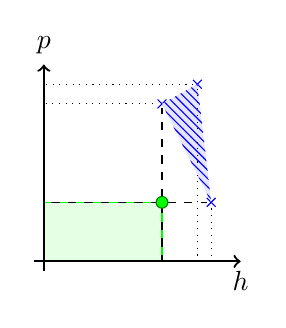
\begin{tikzpicture}[scale=2.5]	
     	
  	\draw (0.85, 0.3) node[cross=2pt,color=blue] (c1) {};
  	\draw (0.78, 0.9) node[cross=2pt,color=blue] (c2) {};
  	\draw (0.6, 0.8) node[cross=2pt,color=blue] (c3) {};
  	
  	\node at (0.6,0.3) (x1) {};
  		\draw[fill=green!10!white,draw=green] (0,0) rectangle (x1);
  		 \draw[thick, ->] (-0.05, 0) -- (1, 0) node[below]{$\rndp$};
  	\draw[thick, ->] (0, -0.05) -- (0, 1) node[above] {$\scp$};

\fill[fill=blue!10] (c1.center)--(c2.center)--(c3.center);
	
	  \fill[fill=blue!20,pattern=north west lines,pattern color=blue] (c1.center)--(c2.center)--(c3.center);
	
  	
  	\draw[dashed] (0,0) |- (c1);
  	\draw[dotted] (0,0) |- (c2);
  	\draw[dotted] (0,0) |- (c3);
  	\draw[dotted] (0,0) -| (c1);
  	\draw[dotted] (0,0) -| (c2);
  	\draw[dashed] (0,0) -| (c3);
  	
  	 
  	\draw (x1) node[circle,fill=green, inner sep=1.5pt,draw=green!50!black] {};
  
  	
  	
\end{tikzpicture}
\caption{Guaranteed points $\solutions_\pOneSched$}
\label{fig:geom:guarantee}
\end{subfigure}
\begin{subfigure}{0.19\textwidth}
\centering
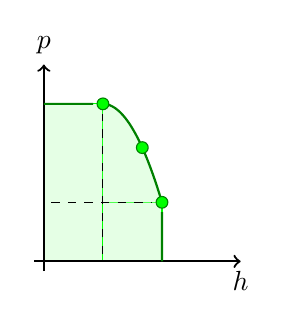
\begin{tikzpicture}[scale=2.5]	
     	
  	\node at (0.6,0.3) (x1) {};
  		\node at (0.3,0.8) (x2) {};
  	
  		\node at (0.5,0.57778) (x3) {};
  	
  		\draw[fill=green!10!white,draw=green] (0,0) rectangle (x1);
  			\draw[fill=green!10!white,draw=green] (0,0) rectangle (x2);
  			
  			
  		 \draw[thick, ->] (-0.05, 0) -- (1, 0) node[below]{$\rndp$};
  	\draw[thick, ->] (0, -0.05) -- (0, 1) node[above] {$\scp$};
  	
  
    \fill[ domain=0.3:0.6, smooth, variable=\x, green!10!white,thick] plot ({\x}, {-5.555*(\x-0.3)*(\x-0.3) + 0.8}) -- (0.3,0.3);
    
  		\draw[name path=f, domain=0.3:0.6, smooth, variable=\x, green!50!black,thick] plot ({\x}, {-5.555*(\x-0.3)*(\x-0.3) + 0.8});
    
  	
  	\draw[dashed] (0,0) -| (x1);
  	\draw[dashed] (0,0) -| (x2);
  	 \draw[dashed] (0,0) |- (x1);
  	\draw[dashed] (0,0) |- (x2);
  	
  		\draw[-,thick,color=green!50!black] (0,0.8) -- (x2);
  	\draw[-,thick,color=green!50!black] (0.6,0.0) -- (x1);
  	 
  	\draw (x1) node[circle,fill=green, inner sep=1.5pt,draw=green!50!black] {};
  \draw (x2) node[circle,fill=green, inner sep=1.5pt,draw=green!50!black] {};
  \draw (x3) node[circle,fill=green, inner sep=1.5pt,draw=green!50!black] {};
  
  
  	
  	
\end{tikzpicture}
\caption{Solutions $\solutions$}
\label{fig:geom:solution}
\end{subfigure}
\begin{subfigure}{0.19\textwidth}
\centering
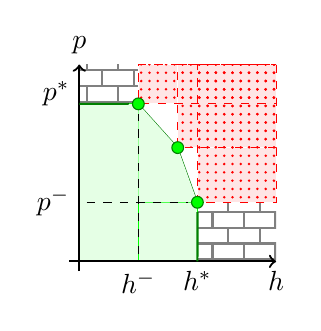
\begin{tikzpicture}[scale=2.5]	
     	
  	\node at (0.6,0.3) (x1) {};
  		\node at (0.3,0.8) (x2) {};
  	
  		\node at (0.5,0.57778) (x3) {};
  		
  					\draw[draw=none,pattern= bricks, pattern color=black!50] (1,0) rectangle (x1);
  					
  					\draw[draw=none,pattern= bricks, pattern color=black!50] (0,1) rectangle (x2);
  	
  		\draw[fill=green!10!white,draw=green] (0,0) rectangle (x1);
  			\draw[fill=green!10!white,draw=green] (0,0) rectangle (x2);
  			
  				\draw[fill=red!10!white,draw=red!0!white] (1,1) rectangle (x1);
  			\draw[fill=red!10!white,draw=red!0!white] (1,1) rectangle (x2);
  					\draw[fill=red!10!white,draw=red!0!white] (1,1) rectangle (x3);
  						\draw[draw=red,dashed] (1,1) rectangle (x1);
  			\draw[draw=red,dashed] (1,1) rectangle (x2);
  					\draw[draw= red,dashed] (1,1) rectangle (x3);
  					
  					\draw[draw=none,dashed,pattern=dots, pattern color=red] (1,1) rectangle (x1);
  					\draw[draw=none,dashed,pattern=dots, pattern color=red] (1,1) rectangle (x2);
  					\draw[draw=none,dashed,pattern=dots, pattern color=red] (1,1) rectangle (x3);
  					
  					
  			
  		 \draw[thick, ->] (-0.05, 0) -- (1, 0) node[below]{$\rndp$};
  	\draw[thick, ->] (0, -0.05) -- (0, 1) node[above] {$\scp$};
  	
  	
  	 \fill[draw=green!50!black] (x2.center) -- (x3.center) -- (x1.center);
    \fill[color=green!10!white] (x2.center) -- (x3.center) -- (x1.center) --  (0.3,0.3);
    
%  		\draw[name path=f, domain=0.3:0.6, smooth, variable=\x, green!50!black,thick] plot ({\x}, {-5.555*(\x-0.3)*(\x-0.3) + 0.8});
%    
  	
  	\draw[dashed] (0,0) -| (x1);
  	\draw[dashed] (0,0) -| (x2);
  	 \draw[dashed] (0,0) |- (x1);
  	\draw[dashed] (0,0) |- (x2);
  	
  		\draw[-,thick,color=green!50!black] (0,0.8) -- (x2);
  	\draw[-,thick,color=green!50!black] (0.6,0.0) -- (x1);
  	 
  	\draw (x1) node[circle,fill=green, inner sep=1.5pt,draw=green!50!black] {};
  \draw (x2) node[circle,fill=green, inner sep=1.5pt,draw=green!50!black] {};
  \draw (x3) node[circle,fill=green, inner sep=1.5pt,draw=green!50!black] {};
  \node[anchor=north] at (0.6,0) {$\rndopt$};
  		
  		\node[anchor=north] at (0.3,0) {$\rndmin$};
  		
  		\node[anchor=east] at (0,0.85) {$\scopt$};
  		
  		\node[anchor=east] at (0,0.3) {$\scmin$};
  
  	
  	
\end{tikzpicture}
\caption{Iterative construction}
\label{fig:geom:iterative}
\end{subfigure}
\begin{subfigure}{0.19\textwidth}
\centering
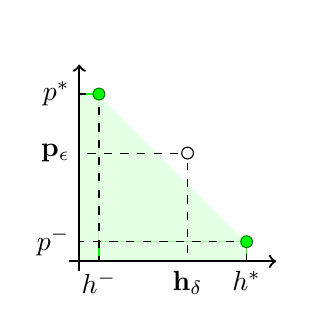
\begin{tikzpicture}[scale=2.5]	
     	
  	\node at (0.85,0.1) (x1) {};
  		\node at (0.1,0.85) (x2) {};
  		
  		\node at (0.55,0.55) (x3) {};
  		
  		\node[anchor=north] at (0.85,0) {$\rndopt$};
  		\node[anchor=north] at (0.55,0) {$\randomness_\delta$};
  		
  		\node[anchor=north] at (0.1,0) {$\rndmin$};
  		
  		\node[anchor=east] at (0,0.85) {$\scopt$};
  		\node[anchor=east] at (0,0.55) {$\scthreshold_\epsilon$};
  		
  		\node[anchor=east] at (0,0.1) {$\scmin$};
  	
  		\draw[fill=green!10!white,draw=green] (0,0) rectangle (x1);
  			\draw[fill=green!10!white,draw=green] (0,0) rectangle (x2);
  			
  			 \fill[draw=white,fill=green!10!white] (x1.center) -- (x2.center) -- (0.1, 0.1);
    
  			
  		 \draw[thick, ->] (-0.05, 0) -- (1, 0) node[below]{\phantom{$\rndp$}};
  	\draw[thick, ->] (0, -0.05) -- (0, 1) node[above] {\phantom{$\scp$}};
  	
  	\draw[dashed] (0,0) -| (x1);
  	\draw[dashed] (0,0) -| (x2);
  	 \draw[dashed] (0,0) |- (x1);
  	\draw[dashed] (0,0) |- (x2);
  	
  	 \draw[dashed] (0,0) |- (x3);
  	\draw[dashed] (0,0) -| (x3);
  	 
  	\draw (x1) node[circle,fill=green, inner sep=1.5pt,draw=green!50!black] {};
  	
  	\draw (x2) node[circle,fill=green, inner sep=1.5pt,draw=green!50!black] {};
  
  	
  	
  	\draw (x3) node[circle,draw,fill=white, inner sep=1.5pt,draw=black] {};
  	
\end{tikzpicture}
\caption{Regret-based ERCI}
\end{subfigure}
\begin{subfigure}{0.19\textwidth}
\centering
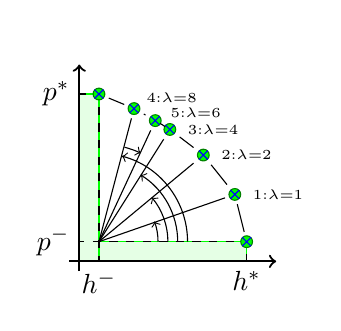
\begin{tikzpicture}[scale=2.5]	
     	
  	\node at (0.85,0.1) (x1) {};
  		\node at (0.1,0.85) (x2) {};
  		
  		
  		\node[anchor=north] at (0.85,0) {$\rndopt$};
  		
  		\node[anchor=north] at (0.1,0) {$\rndmin$};
  		
  		\node[anchor=east] at (0,0.85) {$\scopt$};
  		
  		\node[anchor=east] at (0,0.1) {$\scmin$};
  	
  		\draw[fill=green!10!white,draw=green] (0,0) rectangle (x1);
  			\draw[fill=green!10!white,draw=green] (0,0) rectangle (x2);
  			
  		 \draw[thick, ->] (-0.05, 0) -- (1, 0) node[below]{\phantom{$\rndp$}};
  	\draw[thick, ->] (0, -0.05) -- (0, 1) node[above] {\phantom{$\scp$}};
  	
  	\draw[dashed] (0,0) -| (x1);
  	\draw[dashed] (0,0) -| (x2);
  	 \draw[dashed] (0,0) |- (x1);
  	\draw[dashed] (0,0) |- (x2);
  	
  	 
  	\draw (x1) node[circle,fill=green, inner sep=1.5pt,draw=green!50!black] {};
  	
  	\draw (x2) node[circle,fill=green, inner sep=1.5pt,draw=green!50!black] {};
  	
  	\draw (x1) node[cross=2pt,color=blue] (c3) {};
  	
  	\draw (x2) node[cross=2pt,color=blue] (c3) {};
  
  \draw[black,->] (0.4,0.1) arc (0:20:0.3cm);
  
  		\node at (0.79,0.34) (x3) {};
  			\draw (x3) node[circle,fill=green, inner sep=1.5pt,draw=green!50!black] {};
  			
  	\draw (x3) node[cross=2pt,color=blue] (c3) {};
  	\draw [-] (0.1,0.1) -- (x3);
   \draw[black,->] (0.45,0.1) arc (0:40:0.35cm);
   
   \node at (0.63,0.54) (x4) {};
  			\draw (x4) node[circle,fill=green, inner sep=1.5pt,draw=green!50!black] {};
  			
  	\draw (x4) node[cross=2pt,color=blue] (c3) {};
  	\draw [-] (0.1,0.1) -- (x4);
   
   \draw[black,->] (0.5,0.1) arc (0:58:0.4cm);
    \node at (0.46,0.67) (x5) {};
  			\draw (x5) node[circle,fill=green, inner sep=1.5pt,draw=green!50!black] {};
  			
  	\draw (x5) node[cross=2pt,color=blue] (c3) {};
  	\draw [-] (0.1,0.1) -- (x5);
   \draw[black,->] (0.55,0.1) arc (0:75:0.45cm);
   \node at (0.278,0.776) (x6) {};
  			\draw (x6) node[circle,fill=green, inner sep=1.5pt,draw=green!50!black] {};
  			
  	\draw (x6) node[cross=2pt,color=blue] (c3) {};
  	\draw [-] (0.1,0.1) -- (x6);
  	
   \draw[black,->] (0.23,0.58) arc (75:65:0.5cm);
   \node at (0.386,0.715) (x7) {};
  			\draw (x7) node[circle,fill=green, inner sep=1.5pt,draw=green!50!black] {};
  			
  	\draw (x7) node[cross=2pt,color=blue] (c3) {};
  	\draw [-] (0.1,0.1) -- (x7);

   
   \draw[-] (x1) -- (x3) -- (x4) -- (x5) -- (x7) -- (x6) -- (x2);
   
   \node[anchor=west,xshift=0.3em] at (x3) {\tiny{1:$\lambda{=}1$}};
   \node[anchor=west,xshift=0.3em] at (x4) {\tiny{2:$\lambda{=}2$}};
   \node[anchor=west,xshift=0.3em] at (x5) {\tiny{3:$\lambda{=}4$}};
   \node[anchor=west,yshift=0.3em,xshift=0.2em] at (x7) {\tiny{5:$\lambda{=}6$}};
   \node[anchor=west,yshift=0.4em,xshift=0.1em] at (x6) {\tiny{4:$\lambda{=}8$}};
  	
\end{tikzpicture}
\caption{Rationality-based algorithm}
\end{subfigure}

\caption{Geometric interpretation of the ERCI problem for some fixed SG.}
\end{figure*}
It is convenient to consider this front geometrically.
To begin, given a fixed ERCI instance, a scheduler $\sched$
\emph{induces} a point $x_\sched$:
\begin{equation}
  x_\sched \eqdef \Big\langle \Pr(X_\varphi \mid \sched), H(\sched) \Big\rangle \in [0,1] \times [0,\infty).  
\end{equation}
To ease notation, for $x_\sched = \langle \scp,\rndp \rangle$ we use
$\scp_\sched \eqdef \scp$ and $\rndp_\sched \eqdef \rndp$. Next, we
partially order these points via the standard product ordering:
\begin{equation}
  \langle \scp,\rndp \rangle \preceq \langle \scp',\rndp' \rangle \quad\text{ iff }\quad \scp \leq \scp' \wedge \rndp \leq \rndp'.
\end{equation}

We say that $\pOneSched$ \emph{guarantees} a point $x_\pOne \eqdef
\langle \scp, \rndp \rangle$, if for every policy $\pTwoSched$, using
$\sched = \langle \pOneSched, \pTwoSched \rangle$, we have
$\scp_\sched \geq \scp$ and $\rndp_\sched \geq \rndp$. Thus, a point
is guaranteed if no matter what policy $\pTwo$ uses, $x_\sched$ will
induce a point no worse w.r.t.\ to either randomization or performance
than $x_\pOne$. 
We define
\emph{the set of guaranteed points} for a scheduler $\pOneSched$:
\begin{equation}\label{eq:guaranteed}
  \solutions[\pOneSched] \eqdef \{ \langle \scp, \rndp \rangle \mid  \pOneSched \text{ guarantees } \langle \scp, \rndp \rangle \}.
\end{equation}
We observe that guaranteed points are
downward closed, i.e., if $\pOneSched$ guarantees $x$ and $x' \preceq x$,
then $\pOneSched$ guarantees $x'$.
\begin{example}
Consider Fig.~\ref{fig:geom:guarantee}. We fix $\pOneSched$ and draw all points induced by $\sched = \langle \pOneSched, \pTwoSched \rangle$ when varying $\pTwoSched$ in the blue hatched area. We take the minimal randomness $\rndp$ and the minimal performance $\scp$. The points in the downward closure  of $\langle \scp, \rndp \rangle$ (green circle) are the guaranteed points for $\pOneSched$ in the green solid area.	
We notice the gap between both areas: While the performance and randomization may be better than the optimum that $\pOne$ can guarantee, it cannot guarantee a higher randomization \emph{and} performance simultaneously, as  the $\pTwo$-player would have a counter-policy violating either the performance \emph{or} the randomization.
\end{example}

Points guaranteed by some $\pOneSched$ are called
\emph{achievable}. Thus, the achievable points are: $ \solutions =
\bigcup_{\pOneSched} \solutions[\pOneSched]$.  Importantly, the ERCI problem is realizable iff $\langle \scthreshold,
\randomness \rangle$ is achievable. 
Thus, to solve ERCI instances, we start by characterizing
$\solutions$. We start by observing the $\solutions$ is convex (proof in Sec~\ref{sec:proofs}).


\begin{proposition}\label{prop:convex}
  The set of achievable points, $\solutions$, is convex. 
\end{proposition}

\footnotetext{
  That is, $y, y' \in Y$ implies for
  every $w \in [0,1]$ that $w \cdot y + (1-w) \cdot y \in Y$
}

Next, because $\solutions$ is downward closed, it
suffices to study the ``maximal'' or non-dominated points.  Precisely,
we say that a point $x$ is \emph{dominated} by $x'$ if $x \prec
x'$, i.e., if $x \preceq x' \wedge x \neq x'$.
The Pareto-front $\pareto{\solutions}$ of $\solutions$ is then the set of non-dominated guaranteed points,
\begin{equation}
  \pareto{\solutions} \eqdef \{ x \in \solutions \mid \forall x' \in \solutions, x \not\prec x'  \}.  
\end{equation}
\noindent
\begin{mdframed}
Importantly, it holds that the ERCI problem is satisfiable iff there exists a  $x \in \pareto{\solutions}$ such that $\langle \scthreshold, \randomness \rangle \preceq x$.    
\end{mdframed}
\begin{example}
	The set $\solutions$ illustrated in Fig.~\ref{fig:geom:solution} is obtained by taking the union of guaranteed points, and can be characterized by the set of points on the Pareto-front: This is the curved border between the green and white area, in particular the three green dots are on the Pareto-front. Any ERCI instance with $\langle \scthreshold, \randomness \rangle$ in the green area is realizable.
\end{example}


\noindent
Approximating the Pareto-front gives a natural approximation
scheme for ERCI instances: For any subset $\pareto{} \subseteq
\pareto{\solutions}$,
\begin{enumerate}
\item If there exists an $x \in \pareto{}$ such that
$\langle \scthreshold, \randomness \rangle \preceq x$, then the ERCI
Problem must be realizable, $x$ is a witness to satisfiability.
\item If there exists an $x \in \pareto{}$
such that $x \prec \langle \scthreshold, \randomness \rangle$ then the
ERCI problem is not realizable, and $x$ is a witness to unsatisfiability.
\end{enumerate}
Due to convexity, we may speed up the search for satisfiability: If there exist $x_1, x_2 \in \pareto{}$ such that $\langle \scthreshold, \randomness \rangle \prec \big(w \cdot x_1 + (1-w) \cdot x_2\big)$, we call $x_1,x_2$ a witness-pair.

\begin{example}
\label{ex:approximation}
	Consider Fig.~\ref{fig:geom:iterative}. We have found three points on the Pareto-curve, and already have a good impression of the trade-off between randomization and performance. In particular, the green area is definitively a subset of $\solutions$: It exploits the downward closure and the convexity of $\solutions$. The red (dotted) part contain the points on the Pareto curve in their downward closure, thus they cannot be part of the Pareto curve themselves.
	Furthermore, the topmost point on the Pareto curve was obtained by maximizing performance (and optimizing randomization only as a secondary objective). Thus, by construction, the bricked area at the top is not realizable. Analogously, the bricked area at the right reflects non-achievable randomization. 
\end{example}

Thus a key algorithmic question in ERCI is how to efficiently explore
and approximate the Pareto front $\pareto{\solutions}$. As first steps, we find the two special points induced by (1) optimizing performance and only then randomization (the topmost green point in the figures) and (2) optimizing randomization and only then performance (the rightmost green point). 
As we have seen, these restrict the domain in which we can actually trade performance for randomness. 
We define 
$\rndopt \eqdef \max \{ \rndp \mid \exists \scp \text{ s.t. } \langle \scp, \rndp \rangle \in \solutions  \} $, i.e., the largest randomness that can be guaranteed by any $\pOne$-policy. 
Likewise, we define 
$\scopt \eqdef \max \{ \scp \mid \exists \rndp \text{ s.t. } \langle \scp, \rndp \rangle \in \solutions  \} $, i.e., the largest performance that can be guaranteed by any $\pOne$-policy. 
Then, we define 
$\scmin \eqdef \max \{ \scp \mid \langle \scp, \rndopt \rangle  \in \solutions \}$, the best performance that $\pOne$ can guarantee while guaranteeing optimal randomness. 
Likewise, we define  the analogous $\rndmin \eqdef \max \{ \scp \mid \langle \scp, \rndopt \rangle  \in \solutions \}$.
We thus obtain two points on the Pareto-curve: $\langle \scmin, \rndopt \rangle$ and $\langle \scopt, \rndmin \rangle$, and intuitively, we can trade between these two points following the Pareto curve.

%\begin{remark}[Regret Based ERCI]

Often, rather that fixing $\scthreshold$ and $\randomness$ a
  priori, one seeks to guarantee some percentage of the independently achievable soft
  constraint and causal entropy measure.  We
  re-parameterize ERCI as follows:
  \begin{equation}
    \scthreshold_\epsilon \eqdef \epsilon \cdot (\scopt - \scmin) + \scmin
    \hspace{1em}
    \randomness_\delta \eqdef  \delta \cdot (\rndopt - \rndmin) + \rndmin
  \end{equation}
  where $\epsilon, \delta \in [0, 1]$. We call this version of ERCI \emph{regret-based}. Geometrically, after computing $\scopt$ and $\rndopt$, we know that the left triangle in Fig.~\ref{fig:geom:regret} is definitively realizable, and the regret-based ERCI asks whether the white circle is also realizable (where the point of the white point is given by $\epsilon$ and $\delta$. %As we shall later see, these maximum quantities are
 % directly computed in our proposed algorithm. 
%\end{remark}

Finally, it is helpful to think about the Pareto-curve as a function of randomization in this reparameterization.  We define a characteristic function which given a target
performance ratio, $\epsilon$, yields the optimal randomness ratio,
$\delta$:
\begin{equation}
  \begin{split}
    & \solfuncp\colon [0,1] \rightarrow [0, 1]    \\
    & \solfuncp(\delta) = \max_\epsilon \{ \randomness_\delta \mid \langle
    \scthreshold_\epsilon, \randomness_\delta \rangle \in \solutions \} 
  \end{split}
\end{equation}
\begin{proposition}\label{prop:monotone}
  $\solfuncp$ is continuous and (strictly) decreasing.
\end{proposition}
 We shall temporarily post-pone the proof of
\propref{monotone}. For now, one case observe that
(non-strict) monotone decreasing follows directly from convexity and
using the adequate domains.
Finally, the set  $\solutions$ is (in general) \emph{not} a finite polytope -- the MDP in Fig.~\ref{fig:minimal:mdp} serves as an example. Nevertheless,  $\solutions$ can be well approximated with finitely many vertices, see Ex.~\ref{ex:approximation}.

With these facts, we are now well-equiped to develop the algorithms in Sec.~\ref{sec:mdps} for MDPs and Sec.~\ref{sec:sgs} for SGs.

%%% Local Variables:
%%% mode: latex
%%% TeX-master: "main"
%%% End:



\section{The Control Improvisation Problem for MDPs}
\label{sec:mdps}

We present an algorithm for the control improvisation problem for
MDPs. Recall that an MDP is a stochastic game with a 
The key idea is to rephrase the tradeoff between
randomisation and performance as a degree in rationality $\rat$ of the
policy. Intuitively, a rationality of $\rat = \infty$ means that we
focus completely on the performance criterion, and rationality $\rat =
0$. We can then reuse ideas from maximum entropy inference from
specifications~\cite{DBLP:conf/cav/Vazquez-Chanlatte20}.  In the next
section, we extend this idea to SGs.

\subsection{Rationality}

\noindent
In context of MDPs, the maximum causal entropy policy consistent with
an expected reward (here performance, $\scthreshold$) is given by a
smooth variant of the Bellman equations~\cite{mceThesis}. Namely, let
$\smoothmax{}$ denote the log-sum-exp operator, i.e., $\smoothmax(X)
\eqdef \log \left( \sum_{x\in X} e^x \right)$. For each rationality
$\rat \in [0, \infty)$, we define a policy,
 \begin{align}
   &\sched_\rat(s\mid \act) \eqdef \exp( Q_\rat(s,\act) - V_\rat(s))  \\
   & V_\rat(s) \eqdef  \begin{cases}
     \lambda  \cdot \indicator{s = \target} & \text{if }s \in \{ \target, \sink \},\\
     \smoothmax_{\act \in \EnAct(s)}{  Q_\rat(s,\act) } & \text{otherwise.}
   \end{cases}\\ 
	& Q_\rat(s, \act) \eqdef \sum_{s'} P(s,\act,s') \cdot V_\rat(s').
 \end{align}
\sj{Need to put in enact}
To ease notation, we denote $x_\rat \colonequals x_{\sched_\rat},
\scp_\rat \colonequals \scp_{\sched_\rat}, \rndp_\rat \colonequals
\rndp_{\sched_\rat}$. As previously alluded, the key property
is that $\sched_\rat$ is the \emph{unique} maximum causal entropy policy
such that $\Pr(\varphi) = \scp_\rat$~\cite{DBLP:conf/cav/Vazquez-Chanlatte20}.

In terms of the machinery developed in the previous section, this
family serves to index the Pareto-Front, $\pareto{\solutions}$.  As a
consequence, we can use $\rat$ to explore the Pareto-front.  To see
this, first observe the following easily verified proposition.

\begin{proposition}
  $\scp_\rat$ is smoothly and (strictly) monotonically increasing in $\rat$ and $\rndp_\rat$
  is smoothly (strictly) monotonically decreasing in $\rat$.
\end{proposition}

Intuitively, as $\rat$ approaches $0$, $\sched_\rat$ approaches the
uniform distribution over \emph{all available actions}. Note that this
policy maximizes (causal) entropy, and thus $\rndopt = \rndp_0$.
Similarly, as $\rat$ approaches $\infty$, $\sched_\rat$ selects (uniformly) from
actions \emph{that maximize performance}. Thus, $\scopt = \scp_\infty$.

\subsection{Pareto-exploration}
As a consequence, we can use $\rat$ to explore the Pareto-front.
In particular, assuming $\scopt, \rndopt \neq 0$ (which would
otherwise yield trivial $\solutions$ and $\pareto{\solutions}$), one
can define $\epsilon_\rat \eqdef \nicefrac{\scp_\rat}{\scp_\infty}, \delta_\rat \eqdef \nicefrac{\rndp_\rat}{\rndp_0}$. Then, because
$\sched_\rat$ maximizes randomness given a target performance, one derives:
\begin{equation}
  \solfuncp\left(\epsilon_\rat\right) = \delta_\rat.
\end{equation}
The key algorithmic idea is thus to strategically evaluate a sequence
of rationality coefficients to yield (input, output) pairs for
$\solfuncp$. Due to convexity, the convex hull this sequence of
rationality-indexed points (and the origin) gradually refines a
polygonal approximation of $\solutions$, and thus the Pareto
Front. This approximation, $\hat{\solutions}$, is refined until
either:
\begin{enumerate}
\item $\langle \scthreshold, \randomness \rangle \in \hat{S}$ proving
  $\langle \scthreshold, \randomness \rangle \in \solutions$.
\item A $\rat$ is found such that
  $x_{\rat} \prec \langle \scthreshold, \randomness \rangle$, proving
  $\langle \scthreshold, \randomness \rangle \notin \solutions$.
\end{enumerate}
Next, to extract an improviser, observe that because
$\hat{\solutions}$ is a convex polygon, if $\langle \scthreshold,
\randomness \rangle \in \hat{S}$, then there must two corners of
$\hat{\solutions}$ indexed by $\rat_1$ and $\rat_2$, that form a
triangle with $(0, 0)$ containing $\langle \scthreshold, \randomness
\rangle$. Thus, as in the convexity proof, there must be a convex
combination of $q\cdot x_{\rat_1} + \bar{q}\cdot x_{\rat_2}$ that
dominates $\langle \scthreshold, \randomness \rangle$. Therefore, the
following policy solves the ERCI instance:
\begin{equation}\label{eq:4}
  \sigma^*_\pOne(a\mid s) \eqdef q\cdot \sched_{\rat_1}(a\mid s) + \bar{q} \cdot \sched_{\rat_2}(a \mid s)
\end{equation}

\mypara{Approximation Sequence} The final algorithmic question for
MDPs is then: what order should one evaluate rationality coefficients.
We propose a three staged sequence: (i) Compute $x_\rat$ for the end
points $\rat \in \{0, \infty\}$.  (ii) Double $\rat$ until $h_\rat \leq
\randomness$, yielding $\rat_1\ldots \rat_j$, where $\rat_1 = 1$.
(iii) Binary search for $\rat \in [\rat_{j-1}, \rat{j}]$.
\begin{mdframed}
  Our approximation scheme yields a semi-decision process which halts
  iff either (a) $\langle \scthreshold, \randomness \rangle$ is
  bounded away from $\pareto{\solutions}$ \emph{or} (b)
  $\langle \scthreshold, \randomness \rangle$ is visited by
  $x_{\rat_i}$.
\end{mdframed}
Next, observe that given a maximum resolution, $\kappa$, in
rationality, this approximation scheme becomes linear in the MDP size
and logarithmic in the final rationality coefficient $\rat_*$ and the
resolution $\kappa$, i.e., the run-time is,
\begin{equation}
  O\bigg(\hspace{-1.4em}\underbrace{|\sg|}_{\text{Bellman Backup}}\hspace{-1.4em}\cdot\overbrace{\log(\rat_*)}^{\text{Doubling Phase}}\cdot\underbrace{\log(\nicefrac{1}{\kappa})}_{\text{Binary Search}}\bigg)
\end{equation}
Finally, before generalizing to stochastic games, we observe that in
practice, $\sched_{100} \approx \sched_\infty$, and one can often take
$\rat_* \leq 100$.

%%% Local Variables:
%%% mode: latex
%%% TeX-master: "main"
%%% End:

 
\section{The Control Improvisation Problem for SGs}\label{sec:sgs}
MDP algorithm in hand, we are now ready to provide an algorithm for
stochastic games. At a high level, this algorithm works by initially
planning for $\pTwo$ selecting the action that minimizes randomness
(with ties broken by performance). This assumption leads to a
reduction to the MDP-case, where the rationality indexed family,
$\sched_\rat$, indexes the Pareto Front.  If this assumption is ever
violated, the resulting state must support more randomness.  The
rationality, $\rat$, is thus lowered to match the worst case randomness,
which due to monotonicity of $\solfuncp$, can only increase
performance. Surprisingly, as we shall later prove, this class of
policies indexes the Pareto Front for SGs!

\mypara{Deterministic Adversaries}
First and foremost, observe that to render an ERCI instance
un-achievable, it suffices for $\pTwo$ to violate
either the performance threshold OR the randomness threshold.  Next,
notice that because $\pOneSched$ is a priori fixed, $\pTwoSched$ can
be seen as repeatedly selecting between a convex combination of
$\rndp$ (and $\scp$) for the corresponding sub-graph. As the maximum of a
convex combination is always achievable on the boundaries, we can
w.l.o.g. assume that $\pTwoSched$ is \emph{deterministic}.  Similarly,
notice that given a fixed $\pOneSched$, the worst-case $\pTwoSched$
response can be computed via dynamic programming in topological order
from the leafs to the root of $\sg$.

\mypara{MDP subroutine}
On the other hand, suppose $\pTwoSched$ was known, reducing the SG to
a MDP. As discussed in the previous section, for the MDP case, it
suffices to consider rationality indexed policies. Let use denote the
resulting MDP and maximum causal entropy family of (partial) policies
as $\sg[\pTwoSched]$ and $\pi^\pOne_\rat[\pTwoSched]$ resp. Now
suppose $\rat$ is a priori fixed. Again, via a topological ordered
evaluation of states from the leaves to the root, one can compute the
$\pTwo$ policy, call $\sched_\rat^\pTwo$, that minimizes the maximum
causal entropy policy family, $\pi^\pOne_\rat[~.~]$. By
We shall refer to resulting (partial) schedule as: $\pi_\rat \eqdef \langle
\pi^\pOne_\rat[\sched_\rat^\pTwo] , \sched_\rat^\pTwo \rangle$.

\mypara{Recursively Matching Randomness}
Of course, even if $\rat$ is fixed, $\pTwoSched$ need not be
$\sched^\pTwo_\rat$. Nevertheless, observe that by selecting the worst
entropy MDP, $\pi_\rat$ establishes an achievable randomness for the
sub-game rooted at each state, call $\delta_\rat(s)$. Now suppose,
$\pTwo$ deviates from $\sched_\rat^\pTwo$ at state $s$. Note that, so
long as $\pOneSched$ does not result yield randomness less than
$\delta_\rat(s)$, the worst-case randomness will not decrease.
This begs the question ``what maximum performance can one guarantee at $s' \in
\Succ(s)$ given randomness $\delta_\rat(s)$?''
\begin{mdframed}
  The key observation is that each state $s'$ is the root of a sub
  game, $\sg[s]$, with a corresponding Pareto Front,
  $\pareto{\solutions}[s]$.
\end{mdframed}
In particular, given access the characteristic functions,
$f_\solutions^{s'}$, for each $s' \in \Succ(s)$, one can compute:
\begin{equation}\label{eq:performance_lookup}
  \epsilon_\rat(s) = \min_{s'} f_\solutions^{s'}(\delta_\rat(s)).
\end{equation}
Thus, via dynamic programming, one can define $\epsilon_\rat(\iota)$.
Moreover, assuming that this entropy matching family of policies
indexes $\pareto{\solutions}$ (proved in Lemma ?), one can handle
deviations from $\sigma^\pTwo_\rat$ by ``replanning''. Namely, one
extends $\pi_\rat$ at $s'$ by computing a new rationality coefficient,
$\rat'$, such that:
\begin{equation}
  \delta_{\rat'}(s') = \delta_{\rat}(s)
\end{equation}
Due to the monotonicity $\rat \leq \rat'$, and thus $\epsilon_\rat \leq \epsilon_{\rat'}$, 
Therefore, ignoring the feasibility of computing the exact Pareto
Front, we obtain a synthesis algorithm for SGs!

\mypara{Approximate Pareto Fronts}
Of course, by varying $\rat$, one can only construct approximate
Pareto Fronts. We now
adapt the above algorithm to the case where one has access to
$\kappa$-close Pareto Front under-approximations,
$\hat{f}_\solutions^{s'}$, where $\kappa$ bounds the $\infty$-norm
error. In particular, observe that if $\epsilon_\rat(s)$ is known
within $\kappa$, convex combinations of these intervals cannot
increase the error beyond $\kappa$, i.e.,
\begin{equation}
  q\cdot[x, x + \kappa] + \bar{q}\cdot[y, y + \kappa] = [z, z + \kappa],
\end{equation}
where $z = q\cdot x + \bar{q}\cdot y$. Thus, since $\pi_\rat$ and
$P(s, a)$ are independent of this Pareto Front (and manipulate
performance via convex combinations) the error can only accumulate on
the Pareto Fronts for $s \in S_\pTwo$. Notice then that so long as,
$\kappa\cdot\tau$ is enough resolution to answer $\scp_\rat <
\scthreshold$, one obtains a semi-decision procedure as in the MDP
case.

\begin{mdframed}
  We then propose the following high-level algorithm:
\begin{enumerate}
\item Let $0 < \kappa < 1$ be some arbitrary initial tolerance.
\item Recursively compute $\kappa$-close Pareto Fronts for each state
in $s'$ using causal entropy matching.
\item If $\scthreshold$ is within $\kappa\cdot \tau$ distance to $\hat{\pareto{\solutions}}$,
  halve $\kappa$ and repeat.
\end{enumerate}  
\end{mdframed}
\mypara{Run-time and Decidability}
In practice, this algorithm can be significantly improved by adaptive
tolerances, lazily computing the Pareto Fronts, and only computing
Pareto Fronts for non-deterministic $\pTwo$ states. Nevertheless,
already this na\"ive algorithm gives a sense of the run-time
bottlenecks. Namely, if $\kappa^*$ tolerance is required to terminate,
then the $\kappa$ search introduces $O(\log(\nicefrac{1}{\kappa^*}))$
overhead. Furthermore, by computing $O(|\sg|)$ Pareto fronts, from the
leaves, one ensures that the complexity grows linearly with the graph
size - although the multiplicative constant depends on the number of
rationality coefficients explored per Pareto-front. We found that most
of the rationality coefficients explored were shared, which in
practice seems to amortize the cost per state. Finally, as in the
MDP-case, the resulting algorithm is only a semi-decision procedure,
being decidable if $\langle \scthreshold, \randomness \rangle$ is
bounded away from the root Pareto Front. As the Pareto Front has
measure 0, we argue that this is merely a technical concern, as a
small perturbation to the ERCI instance (i.e. a Smoothed
Analysis~\cite{SmoothedAnalysis}) or $\sg$ admits decidability.

\mypara{Soundness and Completeness} Our algorithm restricts itself to
considering only recursive entropy matching policies,
$\{\sched^{\pOne}_\rat\}_\rat$. Importantly, observe that because
fixing a policy yields a verifiable point in $\solutions$,
we can restrict ourselves to the case in which our algorithm claims
the ERCI instance un-achievable.
Below, we shall assume that our
algorithm claims the ERCI is un-achievable, but there exists
another policy not in $\{\sched^{\pOne}_\rat\}_\rat$, that achieves
$\langle \scthreshold, \randomness \rangle$.

\begin{proof}[Proof Sketch]
  First, observe that on games with only sink nodes, completeness
  follows directly. Now suppose the entropy matching family is
  complete on all sub-graphs of $\sg$ and for the sake of
  contradiction that, assume that,
  \begin{align}
    &\forall \sched_\pOne \in \{\sched^{\pOne}_\rat\}_\rat~.~ x_{\sched_{\pOne}} \prec \langle \scthreshold, \randomness \rangle\label{eq:reject}\\
    &\exists \sched_\pOne^* \notin \{\sched^{\pOne}_\rat\}_\rat~.~  \langle \scthreshold, \randomness \rangle \prec x_{\sched_{\pOne}^*}\label{eq:incomplete}.
  \end{align}
  Let $\sched_\pTwo^*$ denote the min-randomness $\pTwo$-policy given
  $\sched_\pOne^*$. On the MDP, $\sg[\sched_\pTwo^*]$, we know that
  that the soft-bellman backup family is complete, and thus there must
  exist some $\rat$ such that the partial policy $\pi_\rat$ matches
  the worst-case entropy of $\sched_\pOne^*$, i.e.,
  $\rndp_\rat = \rndp_{\sched_\pOne^*}$. Furthermore, because
  $\pi_\rat$ \emph{uniquely} maximizes causal entropy for its
  performance on $\sg[\sched_\pTwo^*]$, $\sched_\pOne^*$ must exactly
  match $\pi_\rat$ on $\sg[\sched_\pTwo^*]$. Thus, these policies must
  differ on some non-minimum entropy sub-graph. By the inductive
  hypothesis, we know that the entropy matching family is complete on
  these subgraphs, and thus if $\sched_\pOne^*$ achieves a given worst
  case performance on this sub graph, there must be an entropy
  matching that does so as well, contradicting
  assumptions~\eqref{eq:reject} and \eqref{eq:incomplete}.  Thus,
  entropy matching must be complete.
\end{proof}

Finally, observe that as a Corollary of the entropy matching family
$\sched^\pOne_\rat$ being complete, it must be the case that
$\solfuncp(\rndp_\rat)$ inherits continuity and (strict) monotonicity
from the MDP case. Namely, at each $\pTwo$ state, the achievable
points $\solutions$ are necessarily the intersection of the achievable
points of the subgraphs. By induction, (with the MDP base case), we
obtain continuity and strict monotonicity.

%%% Local Variables:
%%% mode: latex
%%% TeX-master: "main"
%%% End:

%\begin{mdframed}
%
%\begin{compactenum}
%	\item $\Pr^\sg_{\langle \sched_1,\sched_2 \rangle}(\eventually{h} T) \geq 1$
%	\item $\Pr^\sg_{\langle \sched_1,\sched_2 \rangle}(\eventually{h} G) \geq \lambda$ 
%\end{compactenum}
%\end{mdframed}
%\sj{Define randomly selected policy}
%\sj{Describe in terms of pMDPp}


\section{Implementation and Empirical Evaluation}
\label{sec:empirical}
\begin{figure*}
    \begin{subfigure}{0.47\textwidth}
  \centering
  \scalebox{0.50}{
    %% Creator: Matplotlib, PGF backend
%%
%% To include the figure in your LaTeX document, write
%%   \input{<filename>.pgf}
%%
%% Make sure the required packages are loaded in your preamble
%%   \usepackage{pgf}
%%
%% and, on pdftex
%%   \usepackage[utf8]{inputenc}\DeclareUnicodeCharacter{2212}{-}
%%
%% or, on luatex and xetex
%%   \usepackage{unicode-math}
%%
%% Figures using additional raster images can only be included by \input if
%% they are in the same directory as the main LaTeX file. For loading figures
%% from other directories you can use the `import` package
%%   \usepackage{import}
%%
%% and then include the figures with
%%   \import{<path to file>}{<filename>.pgf}
%%
%% Matplotlib used the following preamble
%%   \usepackage{fontspec}
%%   \setmainfont{DejaVuSerif.ttf}[Path=/home/mvc/.cache/pypoetry/virtualenvs/improvisers-CRyZdLN2-py3.8/lib/python3.8/site-packages/matplotlib/mpl-data/fonts/ttf/]
%%   \setsansfont{DejaVuSans.ttf}[Path=/home/mvc/.cache/pypoetry/virtualenvs/improvisers-CRyZdLN2-py3.8/lib/python3.8/site-packages/matplotlib/mpl-data/fonts/ttf/]
%%   \setmonofont{DejaVuSansMono.ttf}[Path=/home/mvc/.cache/pypoetry/virtualenvs/improvisers-CRyZdLN2-py3.8/lib/python3.8/site-packages/matplotlib/mpl-data/fonts/ttf/]
%%
\begingroup%
\makeatletter%
\begin{pgfpicture}%
\pgfpathrectangle{\pgfpointorigin}{\pgfqpoint{6.000000in}{4.000000in}}%
\pgfusepath{use as bounding box, clip}%
\begin{pgfscope}%
\pgfsetbuttcap%
\pgfsetmiterjoin%
\definecolor{currentfill}{rgb}{1.000000,1.000000,1.000000}%
\pgfsetfillcolor{currentfill}%
\pgfsetlinewidth{0.000000pt}%
\definecolor{currentstroke}{rgb}{1.000000,1.000000,1.000000}%
\pgfsetstrokecolor{currentstroke}%
\pgfsetstrokeopacity{0.000000}%
\pgfsetdash{}{0pt}%
\pgfpathmoveto{\pgfqpoint{0.000000in}{0.000000in}}%
\pgfpathlineto{\pgfqpoint{6.000000in}{0.000000in}}%
\pgfpathlineto{\pgfqpoint{6.000000in}{4.000000in}}%
\pgfpathlineto{\pgfqpoint{0.000000in}{4.000000in}}%
\pgfpathclose%
\pgfusepath{fill}%
\end{pgfscope}%
\begin{pgfscope}%
\pgfsetbuttcap%
\pgfsetmiterjoin%
\definecolor{currentfill}{rgb}{1.000000,1.000000,1.000000}%
\pgfsetfillcolor{currentfill}%
\pgfsetlinewidth{0.000000pt}%
\definecolor{currentstroke}{rgb}{0.000000,0.000000,0.000000}%
\pgfsetstrokecolor{currentstroke}%
\pgfsetstrokeopacity{0.000000}%
\pgfsetdash{}{0pt}%
\pgfpathmoveto{\pgfqpoint{0.750000in}{0.500000in}}%
\pgfpathlineto{\pgfqpoint{5.400000in}{0.500000in}}%
\pgfpathlineto{\pgfqpoint{5.400000in}{3.520000in}}%
\pgfpathlineto{\pgfqpoint{0.750000in}{3.520000in}}%
\pgfpathclose%
\pgfusepath{fill}%
\end{pgfscope}%
\begin{pgfscope}%
\pgfpathrectangle{\pgfqpoint{0.750000in}{0.500000in}}{\pgfqpoint{4.650000in}{3.020000in}}%
\pgfusepath{clip}%
\pgfsetroundcap%
\pgfsetroundjoin%
\pgfsetlinewidth{0.803000pt}%
\definecolor{currentstroke}{rgb}{0.800000,0.800000,0.800000}%
\pgfsetstrokecolor{currentstroke}%
\pgfsetdash{}{0pt}%
\pgfpathmoveto{\pgfqpoint{0.960047in}{0.500000in}}%
\pgfpathlineto{\pgfqpoint{0.960047in}{3.520000in}}%
\pgfusepath{stroke}%
\end{pgfscope}%
\begin{pgfscope}%
\definecolor{textcolor}{rgb}{0.150000,0.150000,0.150000}%
\pgfsetstrokecolor{textcolor}%
\pgfsetfillcolor{textcolor}%
\pgftext[x=0.960047in,y=0.402778in,,top]{\color{textcolor}\sffamily\fontsize{10.000000}{12.000000}\selectfont 0}%
\end{pgfscope}%
\begin{pgfscope}%
\pgfpathrectangle{\pgfqpoint{0.750000in}{0.500000in}}{\pgfqpoint{4.650000in}{3.020000in}}%
\pgfusepath{clip}%
\pgfsetroundcap%
\pgfsetroundjoin%
\pgfsetlinewidth{0.803000pt}%
\definecolor{currentstroke}{rgb}{0.800000,0.800000,0.800000}%
\pgfsetstrokecolor{currentstroke}%
\pgfsetdash{}{0pt}%
\pgfpathmoveto{\pgfqpoint{1.874112in}{0.500000in}}%
\pgfpathlineto{\pgfqpoint{1.874112in}{3.520000in}}%
\pgfusepath{stroke}%
\end{pgfscope}%
\begin{pgfscope}%
\definecolor{textcolor}{rgb}{0.150000,0.150000,0.150000}%
\pgfsetstrokecolor{textcolor}%
\pgfsetfillcolor{textcolor}%
\pgftext[x=1.874112in,y=0.402778in,,top]{\color{textcolor}\sffamily\fontsize{10.000000}{12.000000}\selectfont 50000}%
\end{pgfscope}%
\begin{pgfscope}%
\pgfpathrectangle{\pgfqpoint{0.750000in}{0.500000in}}{\pgfqpoint{4.650000in}{3.020000in}}%
\pgfusepath{clip}%
\pgfsetroundcap%
\pgfsetroundjoin%
\pgfsetlinewidth{0.803000pt}%
\definecolor{currentstroke}{rgb}{0.800000,0.800000,0.800000}%
\pgfsetstrokecolor{currentstroke}%
\pgfsetdash{}{0pt}%
\pgfpathmoveto{\pgfqpoint{2.788176in}{0.500000in}}%
\pgfpathlineto{\pgfqpoint{2.788176in}{3.520000in}}%
\pgfusepath{stroke}%
\end{pgfscope}%
\begin{pgfscope}%
\definecolor{textcolor}{rgb}{0.150000,0.150000,0.150000}%
\pgfsetstrokecolor{textcolor}%
\pgfsetfillcolor{textcolor}%
\pgftext[x=2.788176in,y=0.402778in,,top]{\color{textcolor}\sffamily\fontsize{10.000000}{12.000000}\selectfont 100000}%
\end{pgfscope}%
\begin{pgfscope}%
\pgfpathrectangle{\pgfqpoint{0.750000in}{0.500000in}}{\pgfqpoint{4.650000in}{3.020000in}}%
\pgfusepath{clip}%
\pgfsetroundcap%
\pgfsetroundjoin%
\pgfsetlinewidth{0.803000pt}%
\definecolor{currentstroke}{rgb}{0.800000,0.800000,0.800000}%
\pgfsetstrokecolor{currentstroke}%
\pgfsetdash{}{0pt}%
\pgfpathmoveto{\pgfqpoint{3.702240in}{0.500000in}}%
\pgfpathlineto{\pgfqpoint{3.702240in}{3.520000in}}%
\pgfusepath{stroke}%
\end{pgfscope}%
\begin{pgfscope}%
\definecolor{textcolor}{rgb}{0.150000,0.150000,0.150000}%
\pgfsetstrokecolor{textcolor}%
\pgfsetfillcolor{textcolor}%
\pgftext[x=3.702240in,y=0.402778in,,top]{\color{textcolor}\sffamily\fontsize{10.000000}{12.000000}\selectfont 150000}%
\end{pgfscope}%
\begin{pgfscope}%
\pgfpathrectangle{\pgfqpoint{0.750000in}{0.500000in}}{\pgfqpoint{4.650000in}{3.020000in}}%
\pgfusepath{clip}%
\pgfsetroundcap%
\pgfsetroundjoin%
\pgfsetlinewidth{0.803000pt}%
\definecolor{currentstroke}{rgb}{0.800000,0.800000,0.800000}%
\pgfsetstrokecolor{currentstroke}%
\pgfsetdash{}{0pt}%
\pgfpathmoveto{\pgfqpoint{4.616304in}{0.500000in}}%
\pgfpathlineto{\pgfqpoint{4.616304in}{3.520000in}}%
\pgfusepath{stroke}%
\end{pgfscope}%
\begin{pgfscope}%
\definecolor{textcolor}{rgb}{0.150000,0.150000,0.150000}%
\pgfsetstrokecolor{textcolor}%
\pgfsetfillcolor{textcolor}%
\pgftext[x=4.616304in,y=0.402778in,,top]{\color{textcolor}\sffamily\fontsize{10.000000}{12.000000}\selectfont 200000}%
\end{pgfscope}%
\begin{pgfscope}%
\definecolor{textcolor}{rgb}{0.150000,0.150000,0.150000}%
\pgfsetstrokecolor{textcolor}%
\pgfsetfillcolor{textcolor}%
\pgftext[x=3.075000in,y=0.212809in,,top]{\color{textcolor}\sffamily\fontsize{10.000000}{12.000000}\selectfont BDD nodes ($\approx$ 2.5 $\times$ game states)}%
\end{pgfscope}%
\begin{pgfscope}%
\pgfpathrectangle{\pgfqpoint{0.750000in}{0.500000in}}{\pgfqpoint{4.650000in}{3.020000in}}%
\pgfusepath{clip}%
\pgfsetroundcap%
\pgfsetroundjoin%
\pgfsetlinewidth{0.803000pt}%
\definecolor{currentstroke}{rgb}{0.800000,0.800000,0.800000}%
\pgfsetstrokecolor{currentstroke}%
\pgfsetdash{}{0pt}%
\pgfpathmoveto{\pgfqpoint{0.750000in}{0.636333in}}%
\pgfpathlineto{\pgfqpoint{5.400000in}{0.636333in}}%
\pgfusepath{stroke}%
\end{pgfscope}%
\begin{pgfscope}%
\definecolor{textcolor}{rgb}{0.150000,0.150000,0.150000}%
\pgfsetstrokecolor{textcolor}%
\pgfsetfillcolor{textcolor}%
\pgftext[x=0.564412in, y=0.583571in, left, base]{\color{textcolor}\sffamily\fontsize{10.000000}{12.000000}\selectfont 0}%
\end{pgfscope}%
\begin{pgfscope}%
\pgfpathrectangle{\pgfqpoint{0.750000in}{0.500000in}}{\pgfqpoint{4.650000in}{3.020000in}}%
\pgfusepath{clip}%
\pgfsetroundcap%
\pgfsetroundjoin%
\pgfsetlinewidth{0.803000pt}%
\definecolor{currentstroke}{rgb}{0.800000,0.800000,0.800000}%
\pgfsetstrokecolor{currentstroke}%
\pgfsetdash{}{0pt}%
\pgfpathmoveto{\pgfqpoint{0.750000in}{1.267896in}}%
\pgfpathlineto{\pgfqpoint{5.400000in}{1.267896in}}%
\pgfusepath{stroke}%
\end{pgfscope}%
\begin{pgfscope}%
\definecolor{textcolor}{rgb}{0.150000,0.150000,0.150000}%
\pgfsetstrokecolor{textcolor}%
\pgfsetfillcolor{textcolor}%
\pgftext[x=0.387682in, y=1.215134in, left, base]{\color{textcolor}\sffamily\fontsize{10.000000}{12.000000}\selectfont 100}%
\end{pgfscope}%
\begin{pgfscope}%
\pgfpathrectangle{\pgfqpoint{0.750000in}{0.500000in}}{\pgfqpoint{4.650000in}{3.020000in}}%
\pgfusepath{clip}%
\pgfsetroundcap%
\pgfsetroundjoin%
\pgfsetlinewidth{0.803000pt}%
\definecolor{currentstroke}{rgb}{0.800000,0.800000,0.800000}%
\pgfsetstrokecolor{currentstroke}%
\pgfsetdash{}{0pt}%
\pgfpathmoveto{\pgfqpoint{0.750000in}{1.899459in}}%
\pgfpathlineto{\pgfqpoint{5.400000in}{1.899459in}}%
\pgfusepath{stroke}%
\end{pgfscope}%
\begin{pgfscope}%
\definecolor{textcolor}{rgb}{0.150000,0.150000,0.150000}%
\pgfsetstrokecolor{textcolor}%
\pgfsetfillcolor{textcolor}%
\pgftext[x=0.387682in, y=1.846698in, left, base]{\color{textcolor}\sffamily\fontsize{10.000000}{12.000000}\selectfont 200}%
\end{pgfscope}%
\begin{pgfscope}%
\pgfpathrectangle{\pgfqpoint{0.750000in}{0.500000in}}{\pgfqpoint{4.650000in}{3.020000in}}%
\pgfusepath{clip}%
\pgfsetroundcap%
\pgfsetroundjoin%
\pgfsetlinewidth{0.803000pt}%
\definecolor{currentstroke}{rgb}{0.800000,0.800000,0.800000}%
\pgfsetstrokecolor{currentstroke}%
\pgfsetdash{}{0pt}%
\pgfpathmoveto{\pgfqpoint{0.750000in}{2.531023in}}%
\pgfpathlineto{\pgfqpoint{5.400000in}{2.531023in}}%
\pgfusepath{stroke}%
\end{pgfscope}%
\begin{pgfscope}%
\definecolor{textcolor}{rgb}{0.150000,0.150000,0.150000}%
\pgfsetstrokecolor{textcolor}%
\pgfsetfillcolor{textcolor}%
\pgftext[x=0.387682in, y=2.478261in, left, base]{\color{textcolor}\sffamily\fontsize{10.000000}{12.000000}\selectfont 300}%
\end{pgfscope}%
\begin{pgfscope}%
\pgfpathrectangle{\pgfqpoint{0.750000in}{0.500000in}}{\pgfqpoint{4.650000in}{3.020000in}}%
\pgfusepath{clip}%
\pgfsetroundcap%
\pgfsetroundjoin%
\pgfsetlinewidth{0.803000pt}%
\definecolor{currentstroke}{rgb}{0.800000,0.800000,0.800000}%
\pgfsetstrokecolor{currentstroke}%
\pgfsetdash{}{0pt}%
\pgfpathmoveto{\pgfqpoint{0.750000in}{3.162586in}}%
\pgfpathlineto{\pgfqpoint{5.400000in}{3.162586in}}%
\pgfusepath{stroke}%
\end{pgfscope}%
\begin{pgfscope}%
\definecolor{textcolor}{rgb}{0.150000,0.150000,0.150000}%
\pgfsetstrokecolor{textcolor}%
\pgfsetfillcolor{textcolor}%
\pgftext[x=0.387682in, y=3.109824in, left, base]{\color{textcolor}\sffamily\fontsize{10.000000}{12.000000}\selectfont 400}%
\end{pgfscope}%
\begin{pgfscope}%
\definecolor{textcolor}{rgb}{0.150000,0.150000,0.150000}%
\pgfsetstrokecolor{textcolor}%
\pgfsetfillcolor{textcolor}%
\pgftext[x=0.332126in,y=2.010000in,,bottom,rotate=90.000000]{\color{textcolor}\sffamily\fontsize{10.000000}{12.000000}\selectfont Time to approximate Pareto Front (sec)}%
\end{pgfscope}%
\begin{pgfscope}%
\pgfpathrectangle{\pgfqpoint{0.750000in}{0.500000in}}{\pgfqpoint{4.650000in}{3.020000in}}%
\pgfusepath{clip}%
\pgfsetbuttcap%
\pgfsetroundjoin%
\definecolor{currentfill}{rgb}{0.121569,0.466667,0.705882}%
\pgfsetfillcolor{currentfill}%
\pgfsetfillopacity{0.200000}%
\pgfsetlinewidth{1.003750pt}%
\definecolor{currentstroke}{rgb}{0.121569,0.466667,0.705882}%
\pgfsetstrokecolor{currentstroke}%
\pgfsetstrokeopacity{0.200000}%
\pgfsetdash{}{0pt}%
\pgfsys@defobject{currentmarker}{\pgfqpoint{0.961364in}{0.637273in}}{\pgfqpoint{0.964197in}{0.639408in}}{%
\pgfpathmoveto{\pgfqpoint{0.961364in}{0.637295in}}%
\pgfpathlineto{\pgfqpoint{0.961364in}{0.637273in}}%
\pgfpathlineto{\pgfqpoint{0.964197in}{0.639401in}}%
\pgfpathlineto{\pgfqpoint{0.964197in}{0.639408in}}%
\pgfpathlineto{\pgfqpoint{0.964197in}{0.639408in}}%
\pgfpathlineto{\pgfqpoint{0.961364in}{0.637295in}}%
\pgfpathclose%
\pgfusepath{stroke,fill}%
}%
\begin{pgfscope}%
\pgfsys@transformshift{0.000000in}{0.000000in}%
\pgfsys@useobject{currentmarker}{}%
\end{pgfscope}%
\end{pgfscope}%
\begin{pgfscope}%
\pgfpathrectangle{\pgfqpoint{0.750000in}{0.500000in}}{\pgfqpoint{4.650000in}{3.020000in}}%
\pgfusepath{clip}%
\pgfsetbuttcap%
\pgfsetroundjoin%
\definecolor{currentfill}{rgb}{1.000000,0.498039,0.054902}%
\pgfsetfillcolor{currentfill}%
\pgfsetfillopacity{0.200000}%
\pgfsetlinewidth{1.003750pt}%
\definecolor{currentstroke}{rgb}{1.000000,0.498039,0.054902}%
\pgfsetstrokecolor{currentstroke}%
\pgfsetstrokeopacity{0.200000}%
\pgfsetdash{}{0pt}%
\pgfsys@defobject{currentmarker}{\pgfqpoint{0.961364in}{0.639248in}}{\pgfqpoint{0.964197in}{0.640187in}}{%
\pgfpathmoveto{\pgfqpoint{0.961364in}{0.639755in}}%
\pgfpathlineto{\pgfqpoint{0.961364in}{0.639248in}}%
\pgfpathlineto{\pgfqpoint{0.964197in}{0.639667in}}%
\pgfpathlineto{\pgfqpoint{0.964197in}{0.640187in}}%
\pgfpathlineto{\pgfqpoint{0.964197in}{0.640187in}}%
\pgfpathlineto{\pgfqpoint{0.961364in}{0.639755in}}%
\pgfpathclose%
\pgfusepath{stroke,fill}%
}%
\begin{pgfscope}%
\pgfsys@transformshift{0.000000in}{0.000000in}%
\pgfsys@useobject{currentmarker}{}%
\end{pgfscope}%
\end{pgfscope}%
\begin{pgfscope}%
\pgfpathrectangle{\pgfqpoint{0.750000in}{0.500000in}}{\pgfqpoint{4.650000in}{3.020000in}}%
\pgfusepath{clip}%
\pgfsetbuttcap%
\pgfsetroundjoin%
\definecolor{currentfill}{rgb}{0.121569,0.466667,0.705882}%
\pgfsetfillcolor{currentfill}%
\pgfsetlinewidth{0.481800pt}%
\definecolor{currentstroke}{rgb}{1.000000,1.000000,1.000000}%
\pgfsetstrokecolor{currentstroke}%
\pgfsetdash{}{0pt}%
\pgfsys@defobject{currentmarker}{\pgfqpoint{-0.041667in}{-0.041667in}}{\pgfqpoint{0.041667in}{0.041667in}}{%
\pgfpathmoveto{\pgfqpoint{0.000000in}{-0.041667in}}%
\pgfpathcurveto{\pgfqpoint{0.011050in}{-0.041667in}}{\pgfqpoint{0.021649in}{-0.037276in}}{\pgfqpoint{0.029463in}{-0.029463in}}%
\pgfpathcurveto{\pgfqpoint{0.037276in}{-0.021649in}}{\pgfqpoint{0.041667in}{-0.011050in}}{\pgfqpoint{0.041667in}{0.000000in}}%
\pgfpathcurveto{\pgfqpoint{0.041667in}{0.011050in}}{\pgfqpoint{0.037276in}{0.021649in}}{\pgfqpoint{0.029463in}{0.029463in}}%
\pgfpathcurveto{\pgfqpoint{0.021649in}{0.037276in}}{\pgfqpoint{0.011050in}{0.041667in}}{\pgfqpoint{0.000000in}{0.041667in}}%
\pgfpathcurveto{\pgfqpoint{-0.011050in}{0.041667in}}{\pgfqpoint{-0.021649in}{0.037276in}}{\pgfqpoint{-0.029463in}{0.029463in}}%
\pgfpathcurveto{\pgfqpoint{-0.037276in}{0.021649in}}{\pgfqpoint{-0.041667in}{0.011050in}}{\pgfqpoint{-0.041667in}{0.000000in}}%
\pgfpathcurveto{\pgfqpoint{-0.041667in}{-0.011050in}}{\pgfqpoint{-0.037276in}{-0.021649in}}{\pgfqpoint{-0.029463in}{-0.029463in}}%
\pgfpathcurveto{\pgfqpoint{-0.021649in}{-0.037276in}}{\pgfqpoint{-0.011050in}{-0.041667in}}{\pgfqpoint{0.000000in}{-0.041667in}}%
\pgfpathclose%
\pgfusepath{stroke,fill}%
}%
\begin{pgfscope}%
\pgfsys@transformshift{1.105219in}{0.754121in}%
\pgfsys@useobject{currentmarker}{}%
\end{pgfscope}%
\begin{pgfscope}%
\pgfsys@transformshift{1.201013in}{0.828556in}%
\pgfsys@useobject{currentmarker}{}%
\end{pgfscope}%
\begin{pgfscope}%
\pgfsys@transformshift{1.313607in}{0.925811in}%
\pgfsys@useobject{currentmarker}{}%
\end{pgfscope}%
\begin{pgfscope}%
\pgfsys@transformshift{1.435946in}{1.018527in}%
\pgfsys@useobject{currentmarker}{}%
\end{pgfscope}%
\begin{pgfscope}%
\pgfsys@transformshift{1.564116in}{1.129954in}%
\pgfsys@useobject{currentmarker}{}%
\end{pgfscope}%
\begin{pgfscope}%
\pgfsys@transformshift{1.699434in}{1.259082in}%
\pgfsys@useobject{currentmarker}{}%
\end{pgfscope}%
\begin{pgfscope}%
\pgfsys@transformshift{1.838628in}{1.394207in}%
\pgfsys@useobject{currentmarker}{}%
\end{pgfscope}%
\begin{pgfscope}%
\pgfsys@transformshift{1.981130in}{1.531734in}%
\pgfsys@useobject{currentmarker}{}%
\end{pgfscope}%
\begin{pgfscope}%
\pgfsys@transformshift{0.973283in}{0.652078in}%
\pgfsys@useobject{currentmarker}{}%
\end{pgfscope}%
\begin{pgfscope}%
\pgfsys@transformshift{0.988621in}{0.666943in}%
\pgfsys@useobject{currentmarker}{}%
\end{pgfscope}%
\begin{pgfscope}%
\pgfsys@transformshift{1.032478in}{0.719431in}%
\pgfsys@useobject{currentmarker}{}%
\end{pgfscope}%
\begin{pgfscope}%
\pgfsys@transformshift{1.095512in}{0.723893in}%
\pgfsys@useobject{currentmarker}{}%
\end{pgfscope}%
\begin{pgfscope}%
\pgfsys@transformshift{1.199404in}{0.782613in}%
\pgfsys@useobject{currentmarker}{}%
\end{pgfscope}%
\begin{pgfscope}%
\pgfsys@transformshift{1.326624in}{0.877374in}%
\pgfsys@useobject{currentmarker}{}%
\end{pgfscope}%
\begin{pgfscope}%
\pgfsys@transformshift{1.484958in}{0.955615in}%
\pgfsys@useobject{currentmarker}{}%
\end{pgfscope}%
\begin{pgfscope}%
\pgfsys@transformshift{1.659124in}{1.100753in}%
\pgfsys@useobject{currentmarker}{}%
\end{pgfscope}%
\begin{pgfscope}%
\pgfsys@transformshift{2.235935in}{1.438964in}%
\pgfsys@useobject{currentmarker}{}%
\end{pgfscope}%
\begin{pgfscope}%
\pgfsys@transformshift{3.220876in}{2.113420in}%
\pgfsys@useobject{currentmarker}{}%
\end{pgfscope}%
\begin{pgfscope}%
\pgfsys@transformshift{4.204537in}{2.739110in}%
\pgfsys@useobject{currentmarker}{}%
\end{pgfscope}%
\begin{pgfscope}%
\pgfsys@transformshift{5.188636in}{3.382727in}%
\pgfsys@useobject{currentmarker}{}%
\end{pgfscope}%
\begin{pgfscope}%
\pgfsys@transformshift{0.961364in}{0.637273in}%
\pgfsys@useobject{currentmarker}{}%
\end{pgfscope}%
\begin{pgfscope}%
\pgfsys@transformshift{0.964197in}{0.639401in}%
\pgfsys@useobject{currentmarker}{}%
\end{pgfscope}%
\begin{pgfscope}%
\pgfsys@transformshift{0.974124in}{0.644823in}%
\pgfsys@useobject{currentmarker}{}%
\end{pgfscope}%
\begin{pgfscope}%
\pgfsys@transformshift{0.993246in}{0.653992in}%
\pgfsys@useobject{currentmarker}{}%
\end{pgfscope}%
\begin{pgfscope}%
\pgfsys@transformshift{1.036719in}{0.676435in}%
\pgfsys@useobject{currentmarker}{}%
\end{pgfscope}%
\begin{pgfscope}%
\pgfsys@transformshift{1.102916in}{0.722829in}%
\pgfsys@useobject{currentmarker}{}%
\end{pgfscope}%
\begin{pgfscope}%
\pgfsys@transformshift{1.207868in}{0.776134in}%
\pgfsys@useobject{currentmarker}{}%
\end{pgfscope}%
\begin{pgfscope}%
\pgfsys@transformshift{1.351230in}{0.883244in}%
\pgfsys@useobject{currentmarker}{}%
\end{pgfscope}%
\begin{pgfscope}%
\pgfsys@transformshift{0.961364in}{0.637295in}%
\pgfsys@useobject{currentmarker}{}%
\end{pgfscope}%
\begin{pgfscope}%
\pgfsys@transformshift{0.964197in}{0.639408in}%
\pgfsys@useobject{currentmarker}{}%
\end{pgfscope}%
\begin{pgfscope}%
\pgfsys@transformshift{0.974106in}{0.644281in}%
\pgfsys@useobject{currentmarker}{}%
\end{pgfscope}%
\begin{pgfscope}%
\pgfsys@transformshift{0.991930in}{0.653801in}%
\pgfsys@useobject{currentmarker}{}%
\end{pgfscope}%
\begin{pgfscope}%
\pgfsys@transformshift{1.034617in}{0.751047in}%
\pgfsys@useobject{currentmarker}{}%
\end{pgfscope}%
\begin{pgfscope}%
\pgfsys@transformshift{1.098126in}{0.718782in}%
\pgfsys@useobject{currentmarker}{}%
\end{pgfscope}%
\begin{pgfscope}%
\pgfsys@transformshift{1.207887in}{0.784511in}%
\pgfsys@useobject{currentmarker}{}%
\end{pgfscope}%
\begin{pgfscope}%
\pgfsys@transformshift{1.363918in}{0.896800in}%
\pgfsys@useobject{currentmarker}{}%
\end{pgfscope}%
\end{pgfscope}%
\begin{pgfscope}%
\pgfpathrectangle{\pgfqpoint{0.750000in}{0.500000in}}{\pgfqpoint{4.650000in}{3.020000in}}%
\pgfusepath{clip}%
\pgfsetbuttcap%
\pgfsetroundjoin%
\definecolor{currentfill}{rgb}{1.000000,0.498039,0.054902}%
\pgfsetfillcolor{currentfill}%
\pgfsetlinewidth{0.481800pt}%
\definecolor{currentstroke}{rgb}{1.000000,1.000000,1.000000}%
\pgfsetstrokecolor{currentstroke}%
\pgfsetdash{}{0pt}%
\pgfsys@defobject{currentmarker}{\pgfqpoint{-0.041667in}{-0.041667in}}{\pgfqpoint{0.041667in}{0.041667in}}{%
\pgfpathmoveto{\pgfqpoint{0.000000in}{-0.041667in}}%
\pgfpathcurveto{\pgfqpoint{0.011050in}{-0.041667in}}{\pgfqpoint{0.021649in}{-0.037276in}}{\pgfqpoint{0.029463in}{-0.029463in}}%
\pgfpathcurveto{\pgfqpoint{0.037276in}{-0.021649in}}{\pgfqpoint{0.041667in}{-0.011050in}}{\pgfqpoint{0.041667in}{0.000000in}}%
\pgfpathcurveto{\pgfqpoint{0.041667in}{0.011050in}}{\pgfqpoint{0.037276in}{0.021649in}}{\pgfqpoint{0.029463in}{0.029463in}}%
\pgfpathcurveto{\pgfqpoint{0.021649in}{0.037276in}}{\pgfqpoint{0.011050in}{0.041667in}}{\pgfqpoint{0.000000in}{0.041667in}}%
\pgfpathcurveto{\pgfqpoint{-0.011050in}{0.041667in}}{\pgfqpoint{-0.021649in}{0.037276in}}{\pgfqpoint{-0.029463in}{0.029463in}}%
\pgfpathcurveto{\pgfqpoint{-0.037276in}{0.021649in}}{\pgfqpoint{-0.041667in}{0.011050in}}{\pgfqpoint{-0.041667in}{0.000000in}}%
\pgfpathcurveto{\pgfqpoint{-0.041667in}{-0.011050in}}{\pgfqpoint{-0.037276in}{-0.021649in}}{\pgfqpoint{-0.029463in}{-0.029463in}}%
\pgfpathcurveto{\pgfqpoint{-0.021649in}{-0.037276in}}{\pgfqpoint{-0.011050in}{-0.041667in}}{\pgfqpoint{0.000000in}{-0.041667in}}%
\pgfpathclose%
\pgfusepath{stroke,fill}%
}%
\begin{pgfscope}%
\pgfsys@transformshift{1.105219in}{0.639249in}%
\pgfsys@useobject{currentmarker}{}%
\end{pgfscope}%
\begin{pgfscope}%
\pgfsys@transformshift{1.201013in}{0.639280in}%
\pgfsys@useobject{currentmarker}{}%
\end{pgfscope}%
\begin{pgfscope}%
\pgfsys@transformshift{1.313607in}{0.644556in}%
\pgfsys@useobject{currentmarker}{}%
\end{pgfscope}%
\begin{pgfscope}%
\pgfsys@transformshift{1.435946in}{0.640370in}%
\pgfsys@useobject{currentmarker}{}%
\end{pgfscope}%
\begin{pgfscope}%
\pgfsys@transformshift{1.564116in}{0.640938in}%
\pgfsys@useobject{currentmarker}{}%
\end{pgfscope}%
\begin{pgfscope}%
\pgfsys@transformshift{1.699434in}{0.663616in}%
\pgfsys@useobject{currentmarker}{}%
\end{pgfscope}%
\begin{pgfscope}%
\pgfsys@transformshift{1.838628in}{0.642346in}%
\pgfsys@useobject{currentmarker}{}%
\end{pgfscope}%
\begin{pgfscope}%
\pgfsys@transformshift{1.981130in}{0.643110in}%
\pgfsys@useobject{currentmarker}{}%
\end{pgfscope}%
\begin{pgfscope}%
\pgfsys@transformshift{0.973283in}{0.638892in}%
\pgfsys@useobject{currentmarker}{}%
\end{pgfscope}%
\begin{pgfscope}%
\pgfsys@transformshift{0.988621in}{0.639338in}%
\pgfsys@useobject{currentmarker}{}%
\end{pgfscope}%
\begin{pgfscope}%
\pgfsys@transformshift{1.032478in}{0.639662in}%
\pgfsys@useobject{currentmarker}{}%
\end{pgfscope}%
\begin{pgfscope}%
\pgfsys@transformshift{1.095512in}{0.640149in}%
\pgfsys@useobject{currentmarker}{}%
\end{pgfscope}%
\begin{pgfscope}%
\pgfsys@transformshift{1.199404in}{0.640916in}%
\pgfsys@useobject{currentmarker}{}%
\end{pgfscope}%
\begin{pgfscope}%
\pgfsys@transformshift{1.326624in}{0.641421in}%
\pgfsys@useobject{currentmarker}{}%
\end{pgfscope}%
\begin{pgfscope}%
\pgfsys@transformshift{1.484958in}{0.642190in}%
\pgfsys@useobject{currentmarker}{}%
\end{pgfscope}%
\begin{pgfscope}%
\pgfsys@transformshift{1.659124in}{0.643622in}%
\pgfsys@useobject{currentmarker}{}%
\end{pgfscope}%
\begin{pgfscope}%
\pgfsys@transformshift{2.235935in}{0.646218in}%
\pgfsys@useobject{currentmarker}{}%
\end{pgfscope}%
\begin{pgfscope}%
\pgfsys@transformshift{3.220876in}{0.667886in}%
\pgfsys@useobject{currentmarker}{}%
\end{pgfscope}%
\begin{pgfscope}%
\pgfsys@transformshift{4.204537in}{0.661769in}%
\pgfsys@useobject{currentmarker}{}%
\end{pgfscope}%
\begin{pgfscope}%
\pgfsys@transformshift{5.188636in}{0.675696in}%
\pgfsys@useobject{currentmarker}{}%
\end{pgfscope}%
\begin{pgfscope}%
\pgfsys@transformshift{0.961364in}{0.639248in}%
\pgfsys@useobject{currentmarker}{}%
\end{pgfscope}%
\begin{pgfscope}%
\pgfsys@transformshift{0.964197in}{0.639667in}%
\pgfsys@useobject{currentmarker}{}%
\end{pgfscope}%
\begin{pgfscope}%
\pgfsys@transformshift{0.974124in}{0.640085in}%
\pgfsys@useobject{currentmarker}{}%
\end{pgfscope}%
\begin{pgfscope}%
\pgfsys@transformshift{0.993246in}{0.640643in}%
\pgfsys@useobject{currentmarker}{}%
\end{pgfscope}%
\begin{pgfscope}%
\pgfsys@transformshift{1.036719in}{0.641578in}%
\pgfsys@useobject{currentmarker}{}%
\end{pgfscope}%
\begin{pgfscope}%
\pgfsys@transformshift{1.102916in}{0.642000in}%
\pgfsys@useobject{currentmarker}{}%
\end{pgfscope}%
\begin{pgfscope}%
\pgfsys@transformshift{1.207868in}{0.643092in}%
\pgfsys@useobject{currentmarker}{}%
\end{pgfscope}%
\begin{pgfscope}%
\pgfsys@transformshift{1.351230in}{0.644432in}%
\pgfsys@useobject{currentmarker}{}%
\end{pgfscope}%
\begin{pgfscope}%
\pgfsys@transformshift{0.961364in}{0.639755in}%
\pgfsys@useobject{currentmarker}{}%
\end{pgfscope}%
\begin{pgfscope}%
\pgfsys@transformshift{0.964197in}{0.640187in}%
\pgfsys@useobject{currentmarker}{}%
\end{pgfscope}%
\begin{pgfscope}%
\pgfsys@transformshift{0.974106in}{0.640811in}%
\pgfsys@useobject{currentmarker}{}%
\end{pgfscope}%
\begin{pgfscope}%
\pgfsys@transformshift{0.991930in}{0.641331in}%
\pgfsys@useobject{currentmarker}{}%
\end{pgfscope}%
\begin{pgfscope}%
\pgfsys@transformshift{1.034617in}{0.642092in}%
\pgfsys@useobject{currentmarker}{}%
\end{pgfscope}%
\begin{pgfscope}%
\pgfsys@transformshift{1.098126in}{0.642681in}%
\pgfsys@useobject{currentmarker}{}%
\end{pgfscope}%
\begin{pgfscope}%
\pgfsys@transformshift{1.207887in}{0.644420in}%
\pgfsys@useobject{currentmarker}{}%
\end{pgfscope}%
\begin{pgfscope}%
\pgfsys@transformshift{1.363918in}{0.645614in}%
\pgfsys@useobject{currentmarker}{}%
\end{pgfscope}%
\end{pgfscope}%
\begin{pgfscope}%
\pgfpathrectangle{\pgfqpoint{0.750000in}{0.500000in}}{\pgfqpoint{4.650000in}{3.020000in}}%
\pgfusepath{clip}%
\pgfsetroundcap%
\pgfsetroundjoin%
\pgfsetlinewidth{1.505625pt}%
\definecolor{currentstroke}{rgb}{0.121569,0.466667,0.705882}%
\pgfsetstrokecolor{currentstroke}%
\pgfsetdash{}{0pt}%
\pgfpathmoveto{\pgfqpoint{0.961364in}{0.637284in}}%
\pgfpathlineto{\pgfqpoint{0.964197in}{0.639405in}}%
\pgfpathlineto{\pgfqpoint{0.973283in}{0.652078in}}%
\pgfpathlineto{\pgfqpoint{0.974106in}{0.644281in}}%
\pgfpathlineto{\pgfqpoint{0.974124in}{0.644823in}}%
\pgfpathlineto{\pgfqpoint{0.988621in}{0.666943in}}%
\pgfpathlineto{\pgfqpoint{0.991930in}{0.653801in}}%
\pgfpathlineto{\pgfqpoint{0.993246in}{0.653992in}}%
\pgfpathlineto{\pgfqpoint{1.032478in}{0.719431in}}%
\pgfpathlineto{\pgfqpoint{1.034617in}{0.751047in}}%
\pgfpathlineto{\pgfqpoint{1.036719in}{0.676435in}}%
\pgfpathlineto{\pgfqpoint{1.095512in}{0.723893in}}%
\pgfpathlineto{\pgfqpoint{1.098126in}{0.718782in}}%
\pgfpathlineto{\pgfqpoint{1.102916in}{0.722829in}}%
\pgfpathlineto{\pgfqpoint{1.105219in}{0.754121in}}%
\pgfpathlineto{\pgfqpoint{1.199404in}{0.782613in}}%
\pgfpathlineto{\pgfqpoint{1.201013in}{0.828556in}}%
\pgfpathlineto{\pgfqpoint{1.207868in}{0.776134in}}%
\pgfpathlineto{\pgfqpoint{1.207887in}{0.784511in}}%
\pgfpathlineto{\pgfqpoint{1.313607in}{0.925811in}}%
\pgfpathlineto{\pgfqpoint{1.326624in}{0.877374in}}%
\pgfpathlineto{\pgfqpoint{1.351230in}{0.883244in}}%
\pgfpathlineto{\pgfqpoint{1.363918in}{0.896800in}}%
\pgfpathlineto{\pgfqpoint{1.435946in}{1.018527in}}%
\pgfpathlineto{\pgfqpoint{1.484958in}{0.955615in}}%
\pgfpathlineto{\pgfqpoint{1.564116in}{1.129954in}}%
\pgfpathlineto{\pgfqpoint{1.659124in}{1.100753in}}%
\pgfpathlineto{\pgfqpoint{1.699434in}{1.259082in}}%
\pgfpathlineto{\pgfqpoint{1.838628in}{1.394207in}}%
\pgfpathlineto{\pgfqpoint{1.981130in}{1.531734in}}%
\pgfpathlineto{\pgfqpoint{2.235935in}{1.438964in}}%
\pgfpathlineto{\pgfqpoint{3.220876in}{2.113420in}}%
\pgfpathlineto{\pgfqpoint{4.204537in}{2.739110in}}%
\pgfpathlineto{\pgfqpoint{5.188636in}{3.382727in}}%
\pgfusepath{stroke}%
\end{pgfscope}%
\begin{pgfscope}%
\pgfpathrectangle{\pgfqpoint{0.750000in}{0.500000in}}{\pgfqpoint{4.650000in}{3.020000in}}%
\pgfusepath{clip}%
\pgfsetroundcap%
\pgfsetroundjoin%
\pgfsetlinewidth{1.505625pt}%
\definecolor{currentstroke}{rgb}{1.000000,0.498039,0.054902}%
\pgfsetstrokecolor{currentstroke}%
\pgfsetdash{}{0pt}%
\pgfpathmoveto{\pgfqpoint{0.961364in}{0.639501in}}%
\pgfpathlineto{\pgfqpoint{0.964197in}{0.639927in}}%
\pgfpathlineto{\pgfqpoint{0.973283in}{0.638892in}}%
\pgfpathlineto{\pgfqpoint{0.974106in}{0.640811in}}%
\pgfpathlineto{\pgfqpoint{0.974124in}{0.640085in}}%
\pgfpathlineto{\pgfqpoint{0.988621in}{0.639338in}}%
\pgfpathlineto{\pgfqpoint{0.991930in}{0.641331in}}%
\pgfpathlineto{\pgfqpoint{0.993246in}{0.640643in}}%
\pgfpathlineto{\pgfqpoint{1.032478in}{0.639662in}}%
\pgfpathlineto{\pgfqpoint{1.034617in}{0.642092in}}%
\pgfpathlineto{\pgfqpoint{1.036719in}{0.641578in}}%
\pgfpathlineto{\pgfqpoint{1.095512in}{0.640149in}}%
\pgfpathlineto{\pgfqpoint{1.098126in}{0.642681in}}%
\pgfpathlineto{\pgfqpoint{1.102916in}{0.642000in}}%
\pgfpathlineto{\pgfqpoint{1.105219in}{0.639249in}}%
\pgfpathlineto{\pgfqpoint{1.199404in}{0.640916in}}%
\pgfpathlineto{\pgfqpoint{1.201013in}{0.639280in}}%
\pgfpathlineto{\pgfqpoint{1.207868in}{0.643092in}}%
\pgfpathlineto{\pgfqpoint{1.207887in}{0.644420in}}%
\pgfpathlineto{\pgfqpoint{1.313607in}{0.644556in}}%
\pgfpathlineto{\pgfqpoint{1.326624in}{0.641421in}}%
\pgfpathlineto{\pgfqpoint{1.351230in}{0.644432in}}%
\pgfpathlineto{\pgfqpoint{1.363918in}{0.645614in}}%
\pgfpathlineto{\pgfqpoint{1.435946in}{0.640370in}}%
\pgfpathlineto{\pgfqpoint{1.484958in}{0.642190in}}%
\pgfpathlineto{\pgfqpoint{1.564116in}{0.640938in}}%
\pgfpathlineto{\pgfqpoint{1.659124in}{0.643622in}}%
\pgfpathlineto{\pgfqpoint{1.699434in}{0.663616in}}%
\pgfpathlineto{\pgfqpoint{1.838628in}{0.642346in}}%
\pgfpathlineto{\pgfqpoint{1.981130in}{0.643110in}}%
\pgfpathlineto{\pgfqpoint{2.235935in}{0.646218in}}%
\pgfpathlineto{\pgfqpoint{3.220876in}{0.667886in}}%
\pgfpathlineto{\pgfqpoint{4.204537in}{0.661769in}}%
\pgfpathlineto{\pgfqpoint{5.188636in}{0.675696in}}%
\pgfusepath{stroke}%
\end{pgfscope}%
\begin{pgfscope}%
\pgfsetrectcap%
\pgfsetmiterjoin%
\pgfsetlinewidth{0.803000pt}%
\definecolor{currentstroke}{rgb}{0.800000,0.800000,0.800000}%
\pgfsetstrokecolor{currentstroke}%
\pgfsetdash{}{0pt}%
\pgfpathmoveto{\pgfqpoint{0.750000in}{0.500000in}}%
\pgfpathlineto{\pgfqpoint{0.750000in}{3.520000in}}%
\pgfusepath{stroke}%
\end{pgfscope}%
\begin{pgfscope}%
\pgfsetrectcap%
\pgfsetmiterjoin%
\pgfsetlinewidth{0.803000pt}%
\definecolor{currentstroke}{rgb}{0.800000,0.800000,0.800000}%
\pgfsetstrokecolor{currentstroke}%
\pgfsetdash{}{0pt}%
\pgfpathmoveto{\pgfqpoint{5.400000in}{0.500000in}}%
\pgfpathlineto{\pgfqpoint{5.400000in}{3.520000in}}%
\pgfusepath{stroke}%
\end{pgfscope}%
\begin{pgfscope}%
\pgfsetrectcap%
\pgfsetmiterjoin%
\pgfsetlinewidth{0.803000pt}%
\definecolor{currentstroke}{rgb}{0.800000,0.800000,0.800000}%
\pgfsetstrokecolor{currentstroke}%
\pgfsetdash{}{0pt}%
\pgfpathmoveto{\pgfqpoint{0.750000in}{0.500000in}}%
\pgfpathlineto{\pgfqpoint{5.400000in}{0.500000in}}%
\pgfusepath{stroke}%
\end{pgfscope}%
\begin{pgfscope}%
\pgfsetrectcap%
\pgfsetmiterjoin%
\pgfsetlinewidth{0.803000pt}%
\definecolor{currentstroke}{rgb}{0.800000,0.800000,0.800000}%
\pgfsetstrokecolor{currentstroke}%
\pgfsetdash{}{0pt}%
\pgfpathmoveto{\pgfqpoint{0.750000in}{3.520000in}}%
\pgfpathlineto{\pgfqpoint{5.400000in}{3.520000in}}%
\pgfusepath{stroke}%
\end{pgfscope}%
\begin{pgfscope}%
\definecolor{textcolor}{rgb}{0.150000,0.150000,0.150000}%
\pgfsetstrokecolor{textcolor}%
\pgfsetfillcolor{textcolor}%
\pgftext[x=3.075000in,y=3.603333in,,base]{\color{textcolor}\sffamily\fontsize{12.000000}{14.400000}\selectfont Linear growth in gridworld instances}%
\end{pgfscope}%
\begin{pgfscope}%
\pgfsetbuttcap%
\pgfsetmiterjoin%
\definecolor{currentfill}{rgb}{1.000000,1.000000,1.000000}%
\pgfsetfillcolor{currentfill}%
\pgfsetfillopacity{0.800000}%
\pgfsetlinewidth{1.003750pt}%
\definecolor{currentstroke}{rgb}{0.800000,0.800000,0.800000}%
\pgfsetstrokecolor{currentstroke}%
\pgfsetstrokeopacity{0.800000}%
\pgfsetdash{}{0pt}%
\pgfpathmoveto{\pgfqpoint{0.847222in}{3.001174in}}%
\pgfpathlineto{\pgfqpoint{2.467136in}{3.001174in}}%
\pgfpathquadraticcurveto{\pgfqpoint{2.494914in}{3.001174in}}{\pgfqpoint{2.494914in}{3.028952in}}%
\pgfpathlineto{\pgfqpoint{2.494914in}{3.422778in}}%
\pgfpathquadraticcurveto{\pgfqpoint{2.494914in}{3.450556in}}{\pgfqpoint{2.467136in}{3.450556in}}%
\pgfpathlineto{\pgfqpoint{0.847222in}{3.450556in}}%
\pgfpathquadraticcurveto{\pgfqpoint{0.819444in}{3.450556in}}{\pgfqpoint{0.819444in}{3.422778in}}%
\pgfpathlineto{\pgfqpoint{0.819444in}{3.028952in}}%
\pgfpathquadraticcurveto{\pgfqpoint{0.819444in}{3.001174in}}{\pgfqpoint{0.847222in}{3.001174in}}%
\pgfpathclose%
\pgfusepath{stroke,fill}%
\end{pgfscope}%
\begin{pgfscope}%
\pgfsetroundcap%
\pgfsetroundjoin%
\pgfsetlinewidth{1.505625pt}%
\definecolor{currentstroke}{rgb}{0.121569,0.466667,0.705882}%
\pgfsetstrokecolor{currentstroke}%
\pgfsetdash{}{0pt}%
\pgfpathmoveto{\pgfqpoint{0.875000in}{3.338088in}}%
\pgfpathlineto{\pgfqpoint{1.152778in}{3.338088in}}%
\pgfusepath{stroke}%
\end{pgfscope}%
\begin{pgfscope}%
\definecolor{textcolor}{rgb}{0.150000,0.150000,0.150000}%
\pgfsetstrokecolor{textcolor}%
\pgfsetfillcolor{textcolor}%
\pgftext[x=1.263889in,y=3.289477in,left,base]{\color{textcolor}\sffamily\fontsize{10.000000}{12.000000}\selectfont Solve game time}%
\end{pgfscope}%
\begin{pgfscope}%
\pgfsetroundcap%
\pgfsetroundjoin%
\pgfsetlinewidth{1.505625pt}%
\definecolor{currentstroke}{rgb}{1.000000,0.498039,0.054902}%
\pgfsetstrokecolor{currentstroke}%
\pgfsetdash{}{0pt}%
\pgfpathmoveto{\pgfqpoint{0.875000in}{3.134231in}}%
\pgfpathlineto{\pgfqpoint{1.152778in}{3.134231in}}%
\pgfusepath{stroke}%
\end{pgfscope}%
\begin{pgfscope}%
\definecolor{textcolor}{rgb}{0.150000,0.150000,0.150000}%
\pgfsetstrokecolor{textcolor}%
\pgfsetfillcolor{textcolor}%
\pgftext[x=1.263889in,y=3.085620in,left,base]{\color{textcolor}\sffamily\fontsize{10.000000}{12.000000}\selectfont BDD build time}%
\end{pgfscope}%
\end{pgfpicture}%
\makeatother%
\endgroup%

    }
    \caption{
      Experimental times for computing Pareto Front of a variety
      delivery drone problems\label{fig:exp_times}.
    }
  \end{subfigure}
  \hfill
    \begin{subfigure}{0.47\textwidth}
    \centering \scalebox{0.53}{
      %% Creator: Matplotlib, PGF backend
%%
%% To include the figure in your LaTeX document, write
%%   \input{<filename>.pgf}
%%
%% Make sure the required packages are loaded in your preamble
%%   \usepackage{pgf}
%%
%% and, on pdftex
%%   \usepackage[utf8]{inputenc}\DeclareUnicodeCharacter{2212}{-}
%%
%% or, on luatex and xetex
%%   \usepackage{unicode-math}
%%
%% Figures using additional raster images can only be included by \input if
%% they are in the same directory as the main LaTeX file. For loading figures
%% from other directories you can use the `import` package
%%   \usepackage{import}
%%
%% and then include the figures with
%%   \import{<path to file>}{<filename>.pgf}
%%
%% Matplotlib used the following preamble
%%   \usepackage{fontspec}
%%   \setmainfont{DejaVuSerif.ttf}[Path=/home/mvc/.cache/pypoetry/virtualenvs/improvisers-CRyZdLN2-py3.8/lib/python3.8/site-packages/matplotlib/mpl-data/fonts/ttf/]
%%   \setsansfont{DejaVuSans.ttf}[Path=/home/mvc/.cache/pypoetry/virtualenvs/improvisers-CRyZdLN2-py3.8/lib/python3.8/site-packages/matplotlib/mpl-data/fonts/ttf/]
%%   \setmonofont{DejaVuSansMono.ttf}[Path=/home/mvc/.cache/pypoetry/virtualenvs/improvisers-CRyZdLN2-py3.8/lib/python3.8/site-packages/matplotlib/mpl-data/fonts/ttf/]
%%
\begingroup%
\makeatletter%
\begin{pgfpicture}%
\pgfpathrectangle{\pgfpointorigin}{\pgfqpoint{6.000000in}{4.000000in}}%
\pgfusepath{use as bounding box, clip}%
\begin{pgfscope}%
\pgfsetbuttcap%
\pgfsetmiterjoin%
\definecolor{currentfill}{rgb}{1.000000,1.000000,1.000000}%
\pgfsetfillcolor{currentfill}%
\pgfsetlinewidth{0.000000pt}%
\definecolor{currentstroke}{rgb}{1.000000,1.000000,1.000000}%
\pgfsetstrokecolor{currentstroke}%
\pgfsetstrokeopacity{0.000000}%
\pgfsetdash{}{0pt}%
\pgfpathmoveto{\pgfqpoint{0.000000in}{0.000000in}}%
\pgfpathlineto{\pgfqpoint{6.000000in}{0.000000in}}%
\pgfpathlineto{\pgfqpoint{6.000000in}{4.000000in}}%
\pgfpathlineto{\pgfqpoint{0.000000in}{4.000000in}}%
\pgfpathclose%
\pgfusepath{fill}%
\end{pgfscope}%
\begin{pgfscope}%
\pgfsetbuttcap%
\pgfsetmiterjoin%
\definecolor{currentfill}{rgb}{1.000000,1.000000,1.000000}%
\pgfsetfillcolor{currentfill}%
\pgfsetlinewidth{0.000000pt}%
\definecolor{currentstroke}{rgb}{0.000000,0.000000,0.000000}%
\pgfsetstrokecolor{currentstroke}%
\pgfsetstrokeopacity{0.000000}%
\pgfsetdash{}{0pt}%
\pgfpathmoveto{\pgfqpoint{0.965972in}{0.580556in}}%
\pgfpathlineto{\pgfqpoint{5.850000in}{0.580556in}}%
\pgfpathlineto{\pgfqpoint{5.850000in}{3.627778in}}%
\pgfpathlineto{\pgfqpoint{0.965972in}{3.627778in}}%
\pgfpathclose%
\pgfusepath{fill}%
\end{pgfscope}%
\begin{pgfscope}%
\pgfpathrectangle{\pgfqpoint{0.965972in}{0.580556in}}{\pgfqpoint{4.884028in}{3.047222in}}%
\pgfusepath{clip}%
\pgfsetroundcap%
\pgfsetroundjoin%
\pgfsetlinewidth{0.803000pt}%
\definecolor{currentstroke}{rgb}{0.800000,0.800000,0.800000}%
\pgfsetstrokecolor{currentstroke}%
\pgfsetdash{}{0pt}%
\pgfpathmoveto{\pgfqpoint{1.187973in}{0.580556in}}%
\pgfpathlineto{\pgfqpoint{1.187973in}{3.627778in}}%
\pgfusepath{stroke}%
\end{pgfscope}%
\begin{pgfscope}%
\definecolor{textcolor}{rgb}{0.150000,0.150000,0.150000}%
\pgfsetstrokecolor{textcolor}%
\pgfsetfillcolor{textcolor}%
\pgftext[x=1.187973in,y=0.483333in,,top]{\color{textcolor}\sffamily\fontsize{10.000000}{12.000000}\selectfont 10}%
\end{pgfscope}%
\begin{pgfscope}%
\pgfpathrectangle{\pgfqpoint{0.965972in}{0.580556in}}{\pgfqpoint{4.884028in}{3.047222in}}%
\pgfusepath{clip}%
\pgfsetroundcap%
\pgfsetroundjoin%
\pgfsetlinewidth{0.803000pt}%
\definecolor{currentstroke}{rgb}{0.800000,0.800000,0.800000}%
\pgfsetstrokecolor{currentstroke}%
\pgfsetdash{}{0pt}%
\pgfpathmoveto{\pgfqpoint{1.927978in}{0.580556in}}%
\pgfpathlineto{\pgfqpoint{1.927978in}{3.627778in}}%
\pgfusepath{stroke}%
\end{pgfscope}%
\begin{pgfscope}%
\definecolor{textcolor}{rgb}{0.150000,0.150000,0.150000}%
\pgfsetstrokecolor{textcolor}%
\pgfsetfillcolor{textcolor}%
\pgftext[x=1.927978in,y=0.483333in,,top]{\color{textcolor}\sffamily\fontsize{10.000000}{12.000000}\selectfont 15}%
\end{pgfscope}%
\begin{pgfscope}%
\pgfpathrectangle{\pgfqpoint{0.965972in}{0.580556in}}{\pgfqpoint{4.884028in}{3.047222in}}%
\pgfusepath{clip}%
\pgfsetroundcap%
\pgfsetroundjoin%
\pgfsetlinewidth{0.803000pt}%
\definecolor{currentstroke}{rgb}{0.800000,0.800000,0.800000}%
\pgfsetstrokecolor{currentstroke}%
\pgfsetdash{}{0pt}%
\pgfpathmoveto{\pgfqpoint{2.667982in}{0.580556in}}%
\pgfpathlineto{\pgfqpoint{2.667982in}{3.627778in}}%
\pgfusepath{stroke}%
\end{pgfscope}%
\begin{pgfscope}%
\definecolor{textcolor}{rgb}{0.150000,0.150000,0.150000}%
\pgfsetstrokecolor{textcolor}%
\pgfsetfillcolor{textcolor}%
\pgftext[x=2.667982in,y=0.483333in,,top]{\color{textcolor}\sffamily\fontsize{10.000000}{12.000000}\selectfont 20}%
\end{pgfscope}%
\begin{pgfscope}%
\pgfpathrectangle{\pgfqpoint{0.965972in}{0.580556in}}{\pgfqpoint{4.884028in}{3.047222in}}%
\pgfusepath{clip}%
\pgfsetroundcap%
\pgfsetroundjoin%
\pgfsetlinewidth{0.803000pt}%
\definecolor{currentstroke}{rgb}{0.800000,0.800000,0.800000}%
\pgfsetstrokecolor{currentstroke}%
\pgfsetdash{}{0pt}%
\pgfpathmoveto{\pgfqpoint{3.407986in}{0.580556in}}%
\pgfpathlineto{\pgfqpoint{3.407986in}{3.627778in}}%
\pgfusepath{stroke}%
\end{pgfscope}%
\begin{pgfscope}%
\definecolor{textcolor}{rgb}{0.150000,0.150000,0.150000}%
\pgfsetstrokecolor{textcolor}%
\pgfsetfillcolor{textcolor}%
\pgftext[x=3.407986in,y=0.483333in,,top]{\color{textcolor}\sffamily\fontsize{10.000000}{12.000000}\selectfont 25}%
\end{pgfscope}%
\begin{pgfscope}%
\pgfpathrectangle{\pgfqpoint{0.965972in}{0.580556in}}{\pgfqpoint{4.884028in}{3.047222in}}%
\pgfusepath{clip}%
\pgfsetroundcap%
\pgfsetroundjoin%
\pgfsetlinewidth{0.803000pt}%
\definecolor{currentstroke}{rgb}{0.800000,0.800000,0.800000}%
\pgfsetstrokecolor{currentstroke}%
\pgfsetdash{}{0pt}%
\pgfpathmoveto{\pgfqpoint{4.147990in}{0.580556in}}%
\pgfpathlineto{\pgfqpoint{4.147990in}{3.627778in}}%
\pgfusepath{stroke}%
\end{pgfscope}%
\begin{pgfscope}%
\definecolor{textcolor}{rgb}{0.150000,0.150000,0.150000}%
\pgfsetstrokecolor{textcolor}%
\pgfsetfillcolor{textcolor}%
\pgftext[x=4.147990in,y=0.483333in,,top]{\color{textcolor}\sffamily\fontsize{10.000000}{12.000000}\selectfont 30}%
\end{pgfscope}%
\begin{pgfscope}%
\pgfpathrectangle{\pgfqpoint{0.965972in}{0.580556in}}{\pgfqpoint{4.884028in}{3.047222in}}%
\pgfusepath{clip}%
\pgfsetroundcap%
\pgfsetroundjoin%
\pgfsetlinewidth{0.803000pt}%
\definecolor{currentstroke}{rgb}{0.800000,0.800000,0.800000}%
\pgfsetstrokecolor{currentstroke}%
\pgfsetdash{}{0pt}%
\pgfpathmoveto{\pgfqpoint{4.887995in}{0.580556in}}%
\pgfpathlineto{\pgfqpoint{4.887995in}{3.627778in}}%
\pgfusepath{stroke}%
\end{pgfscope}%
\begin{pgfscope}%
\definecolor{textcolor}{rgb}{0.150000,0.150000,0.150000}%
\pgfsetstrokecolor{textcolor}%
\pgfsetfillcolor{textcolor}%
\pgftext[x=4.887995in,y=0.483333in,,top]{\color{textcolor}\sffamily\fontsize{10.000000}{12.000000}\selectfont 35}%
\end{pgfscope}%
\begin{pgfscope}%
\pgfpathrectangle{\pgfqpoint{0.965972in}{0.580556in}}{\pgfqpoint{4.884028in}{3.047222in}}%
\pgfusepath{clip}%
\pgfsetroundcap%
\pgfsetroundjoin%
\pgfsetlinewidth{0.803000pt}%
\definecolor{currentstroke}{rgb}{0.800000,0.800000,0.800000}%
\pgfsetstrokecolor{currentstroke}%
\pgfsetdash{}{0pt}%
\pgfpathmoveto{\pgfqpoint{5.627999in}{0.580556in}}%
\pgfpathlineto{\pgfqpoint{5.627999in}{3.627778in}}%
\pgfusepath{stroke}%
\end{pgfscope}%
\begin{pgfscope}%
\definecolor{textcolor}{rgb}{0.150000,0.150000,0.150000}%
\pgfsetstrokecolor{textcolor}%
\pgfsetfillcolor{textcolor}%
\pgftext[x=5.627999in,y=0.483333in,,top]{\color{textcolor}\sffamily\fontsize{10.000000}{12.000000}\selectfont 40}%
\end{pgfscope}%
\begin{pgfscope}%
\definecolor{textcolor}{rgb}{0.150000,0.150000,0.150000}%
\pgfsetstrokecolor{textcolor}%
\pgfsetfillcolor{textcolor}%
\pgftext[x=3.407986in,y=0.293365in,,top]{\color{textcolor}\sffamily\fontsize{10.000000}{12.000000}\selectfont horizon}%
\end{pgfscope}%
\begin{pgfscope}%
\pgfpathrectangle{\pgfqpoint{0.965972in}{0.580556in}}{\pgfqpoint{4.884028in}{3.047222in}}%
\pgfusepath{clip}%
\pgfsetroundcap%
\pgfsetroundjoin%
\pgfsetlinewidth{0.803000pt}%
\definecolor{currentstroke}{rgb}{0.800000,0.800000,0.800000}%
\pgfsetstrokecolor{currentstroke}%
\pgfsetdash{}{0pt}%
\pgfpathmoveto{\pgfqpoint{0.965972in}{0.580556in}}%
\pgfpathlineto{\pgfqpoint{5.850000in}{0.580556in}}%
\pgfusepath{stroke}%
\end{pgfscope}%
\begin{pgfscope}%
\definecolor{textcolor}{rgb}{0.150000,0.150000,0.150000}%
\pgfsetstrokecolor{textcolor}%
\pgfsetfillcolor{textcolor}%
\pgftext[x=0.780385in, y=0.527794in, left, base]{\color{textcolor}\sffamily\fontsize{10.000000}{12.000000}\selectfont 0}%
\end{pgfscope}%
\begin{pgfscope}%
\pgfpathrectangle{\pgfqpoint{0.965972in}{0.580556in}}{\pgfqpoint{4.884028in}{3.047222in}}%
\pgfusepath{clip}%
\pgfsetroundcap%
\pgfsetroundjoin%
\pgfsetlinewidth{0.803000pt}%
\definecolor{currentstroke}{rgb}{0.800000,0.800000,0.800000}%
\pgfsetstrokecolor{currentstroke}%
\pgfsetdash{}{0pt}%
\pgfpathmoveto{\pgfqpoint{0.965972in}{1.088426in}}%
\pgfpathlineto{\pgfqpoint{5.850000in}{1.088426in}}%
\pgfusepath{stroke}%
\end{pgfscope}%
\begin{pgfscope}%
\definecolor{textcolor}{rgb}{0.150000,0.150000,0.150000}%
\pgfsetstrokecolor{textcolor}%
\pgfsetfillcolor{textcolor}%
\pgftext[x=0.426923in, y=1.035664in, left, base]{\color{textcolor}\sffamily\fontsize{10.000000}{12.000000}\selectfont 50000}%
\end{pgfscope}%
\begin{pgfscope}%
\pgfpathrectangle{\pgfqpoint{0.965972in}{0.580556in}}{\pgfqpoint{4.884028in}{3.047222in}}%
\pgfusepath{clip}%
\pgfsetroundcap%
\pgfsetroundjoin%
\pgfsetlinewidth{0.803000pt}%
\definecolor{currentstroke}{rgb}{0.800000,0.800000,0.800000}%
\pgfsetstrokecolor{currentstroke}%
\pgfsetdash{}{0pt}%
\pgfpathmoveto{\pgfqpoint{0.965972in}{1.596296in}}%
\pgfpathlineto{\pgfqpoint{5.850000in}{1.596296in}}%
\pgfusepath{stroke}%
\end{pgfscope}%
\begin{pgfscope}%
\definecolor{textcolor}{rgb}{0.150000,0.150000,0.150000}%
\pgfsetstrokecolor{textcolor}%
\pgfsetfillcolor{textcolor}%
\pgftext[x=0.338558in, y=1.543535in, left, base]{\color{textcolor}\sffamily\fontsize{10.000000}{12.000000}\selectfont 100000}%
\end{pgfscope}%
\begin{pgfscope}%
\pgfpathrectangle{\pgfqpoint{0.965972in}{0.580556in}}{\pgfqpoint{4.884028in}{3.047222in}}%
\pgfusepath{clip}%
\pgfsetroundcap%
\pgfsetroundjoin%
\pgfsetlinewidth{0.803000pt}%
\definecolor{currentstroke}{rgb}{0.800000,0.800000,0.800000}%
\pgfsetstrokecolor{currentstroke}%
\pgfsetdash{}{0pt}%
\pgfpathmoveto{\pgfqpoint{0.965972in}{2.104167in}}%
\pgfpathlineto{\pgfqpoint{5.850000in}{2.104167in}}%
\pgfusepath{stroke}%
\end{pgfscope}%
\begin{pgfscope}%
\definecolor{textcolor}{rgb}{0.150000,0.150000,0.150000}%
\pgfsetstrokecolor{textcolor}%
\pgfsetfillcolor{textcolor}%
\pgftext[x=0.338558in, y=2.051405in, left, base]{\color{textcolor}\sffamily\fontsize{10.000000}{12.000000}\selectfont 150000}%
\end{pgfscope}%
\begin{pgfscope}%
\pgfpathrectangle{\pgfqpoint{0.965972in}{0.580556in}}{\pgfqpoint{4.884028in}{3.047222in}}%
\pgfusepath{clip}%
\pgfsetroundcap%
\pgfsetroundjoin%
\pgfsetlinewidth{0.803000pt}%
\definecolor{currentstroke}{rgb}{0.800000,0.800000,0.800000}%
\pgfsetstrokecolor{currentstroke}%
\pgfsetdash{}{0pt}%
\pgfpathmoveto{\pgfqpoint{0.965972in}{2.612037in}}%
\pgfpathlineto{\pgfqpoint{5.850000in}{2.612037in}}%
\pgfusepath{stroke}%
\end{pgfscope}%
\begin{pgfscope}%
\definecolor{textcolor}{rgb}{0.150000,0.150000,0.150000}%
\pgfsetstrokecolor{textcolor}%
\pgfsetfillcolor{textcolor}%
\pgftext[x=0.338558in, y=2.559276in, left, base]{\color{textcolor}\sffamily\fontsize{10.000000}{12.000000}\selectfont 200000}%
\end{pgfscope}%
\begin{pgfscope}%
\pgfpathrectangle{\pgfqpoint{0.965972in}{0.580556in}}{\pgfqpoint{4.884028in}{3.047222in}}%
\pgfusepath{clip}%
\pgfsetroundcap%
\pgfsetroundjoin%
\pgfsetlinewidth{0.803000pt}%
\definecolor{currentstroke}{rgb}{0.800000,0.800000,0.800000}%
\pgfsetstrokecolor{currentstroke}%
\pgfsetdash{}{0pt}%
\pgfpathmoveto{\pgfqpoint{0.965972in}{3.119907in}}%
\pgfpathlineto{\pgfqpoint{5.850000in}{3.119907in}}%
\pgfusepath{stroke}%
\end{pgfscope}%
\begin{pgfscope}%
\definecolor{textcolor}{rgb}{0.150000,0.150000,0.150000}%
\pgfsetstrokecolor{textcolor}%
\pgfsetfillcolor{textcolor}%
\pgftext[x=0.338558in, y=3.067146in, left, base]{\color{textcolor}\sffamily\fontsize{10.000000}{12.000000}\selectfont 250000}%
\end{pgfscope}%
\begin{pgfscope}%
\pgfpathrectangle{\pgfqpoint{0.965972in}{0.580556in}}{\pgfqpoint{4.884028in}{3.047222in}}%
\pgfusepath{clip}%
\pgfsetroundcap%
\pgfsetroundjoin%
\pgfsetlinewidth{0.803000pt}%
\definecolor{currentstroke}{rgb}{0.800000,0.800000,0.800000}%
\pgfsetstrokecolor{currentstroke}%
\pgfsetdash{}{0pt}%
\pgfpathmoveto{\pgfqpoint{0.965972in}{3.627778in}}%
\pgfpathlineto{\pgfqpoint{5.850000in}{3.627778in}}%
\pgfusepath{stroke}%
\end{pgfscope}%
\begin{pgfscope}%
\definecolor{textcolor}{rgb}{0.150000,0.150000,0.150000}%
\pgfsetstrokecolor{textcolor}%
\pgfsetfillcolor{textcolor}%
\pgftext[x=0.338558in, y=3.575016in, left, base]{\color{textcolor}\sffamily\fontsize{10.000000}{12.000000}\selectfont 300000}%
\end{pgfscope}%
\begin{pgfscope}%
\definecolor{textcolor}{rgb}{0.150000,0.150000,0.150000}%
\pgfsetstrokecolor{textcolor}%
\pgfsetfillcolor{textcolor}%
\pgftext[x=0.283002in,y=2.104167in,,bottom,rotate=90.000000]{\color{textcolor}\sffamily\fontsize{10.000000}{12.000000}\selectfont BDD nodes ($\approx$ 2 × game states)}%
\end{pgfscope}%
\begin{pgfscope}%
\pgfpathrectangle{\pgfqpoint{0.965972in}{0.580556in}}{\pgfqpoint{4.884028in}{3.047222in}}%
\pgfusepath{clip}%
\pgfsetroundcap%
\pgfsetroundjoin%
\pgfsetlinewidth{1.505625pt}%
\definecolor{currentstroke}{rgb}{0.400000,0.760784,0.647059}%
\pgfsetstrokecolor{currentstroke}%
\pgfsetdash{}{0pt}%
\pgfpathmoveto{\pgfqpoint{1.187973in}{0.661216in}}%
\pgfpathlineto{\pgfqpoint{1.335974in}{0.714440in}}%
\pgfpathlineto{\pgfqpoint{1.483975in}{0.777000in}}%
\pgfpathlineto{\pgfqpoint{1.631976in}{0.844973in}}%
\pgfpathlineto{\pgfqpoint{1.779977in}{0.916187in}}%
\pgfpathlineto{\pgfqpoint{1.927978in}{0.991372in}}%
\pgfpathlineto{\pgfqpoint{2.075979in}{1.068710in}}%
\pgfpathlineto{\pgfqpoint{2.223979in}{1.147887in}}%
\pgfusepath{stroke}%
\end{pgfscope}%
\begin{pgfscope}%
\pgfpathrectangle{\pgfqpoint{0.965972in}{0.580556in}}{\pgfqpoint{4.884028in}{3.047222in}}%
\pgfusepath{clip}%
\pgfsetroundcap%
\pgfsetroundjoin%
\pgfsetlinewidth{1.505625pt}%
\definecolor{currentstroke}{rgb}{0.988235,0.552941,0.384314}%
\pgfsetstrokecolor{currentstroke}%
\pgfsetdash{}{0pt}%
\pgfpathmoveto{\pgfqpoint{1.187973in}{0.587910in}}%
\pgfpathlineto{\pgfqpoint{1.335974in}{0.596432in}}%
\pgfpathlineto{\pgfqpoint{1.483975in}{0.620799in}}%
\pgfpathlineto{\pgfqpoint{1.631976in}{0.655822in}}%
\pgfpathlineto{\pgfqpoint{1.779977in}{0.713546in}}%
\pgfpathlineto{\pgfqpoint{1.927978in}{0.784232in}}%
\pgfpathlineto{\pgfqpoint{2.075979in}{0.872205in}}%
\pgfpathlineto{\pgfqpoint{2.223979in}{0.968975in}}%
\pgfpathlineto{\pgfqpoint{2.667982in}{1.289461in}}%
\pgfpathlineto{\pgfqpoint{3.407986in}{1.836712in}}%
\pgfpathlineto{\pgfqpoint{4.147990in}{2.383252in}}%
\pgfpathlineto{\pgfqpoint{4.887995in}{2.930035in}}%
\pgfusepath{stroke}%
\end{pgfscope}%
\begin{pgfscope}%
\pgfpathrectangle{\pgfqpoint{0.965972in}{0.580556in}}{\pgfqpoint{4.884028in}{3.047222in}}%
\pgfusepath{clip}%
\pgfsetroundcap%
\pgfsetroundjoin%
\pgfsetlinewidth{1.505625pt}%
\definecolor{currentstroke}{rgb}{0.552941,0.627451,0.796078}%
\pgfsetstrokecolor{currentstroke}%
\pgfsetdash{}{0pt}%
\pgfpathmoveto{\pgfqpoint{1.187973in}{0.581287in}}%
\pgfpathlineto{\pgfqpoint{1.335974in}{0.582861in}}%
\pgfpathlineto{\pgfqpoint{1.483975in}{0.588377in}}%
\pgfpathlineto{\pgfqpoint{1.631976in}{0.599001in}}%
\pgfpathlineto{\pgfqpoint{1.779977in}{0.623156in}}%
\pgfpathlineto{\pgfqpoint{1.927978in}{0.659936in}}%
\pgfpathlineto{\pgfqpoint{2.075979in}{0.718249in}}%
\pgfpathlineto{\pgfqpoint{2.223979in}{0.797904in}}%
\pgfusepath{stroke}%
\end{pgfscope}%
\begin{pgfscope}%
\pgfpathrectangle{\pgfqpoint{0.965972in}{0.580556in}}{\pgfqpoint{4.884028in}{3.047222in}}%
\pgfusepath{clip}%
\pgfsetroundcap%
\pgfsetroundjoin%
\pgfsetlinewidth{1.505625pt}%
\definecolor{currentstroke}{rgb}{0.905882,0.541176,0.764706}%
\pgfsetstrokecolor{currentstroke}%
\pgfsetdash{}{0pt}%
\pgfpathmoveto{\pgfqpoint{1.187973in}{0.581287in}}%
\pgfpathlineto{\pgfqpoint{1.335974in}{0.582861in}}%
\pgfpathlineto{\pgfqpoint{1.483975in}{0.588367in}}%
\pgfpathlineto{\pgfqpoint{1.631976in}{0.598270in}}%
\pgfpathlineto{\pgfqpoint{1.779977in}{0.621988in}}%
\pgfpathlineto{\pgfqpoint{1.927978in}{0.657274in}}%
\pgfpathlineto{\pgfqpoint{2.075979in}{0.718260in}}%
\pgfpathlineto{\pgfqpoint{2.223979in}{0.804953in}}%
\pgfpathlineto{\pgfqpoint{4.147990in}{3.446102in}}%
\pgfpathlineto{\pgfqpoint{4.275774in}{3.641667in}}%
\pgfusepath{stroke}%
\end{pgfscope}%
\begin{pgfscope}%
\pgfsetrectcap%
\pgfsetmiterjoin%
\pgfsetlinewidth{0.803000pt}%
\definecolor{currentstroke}{rgb}{0.800000,0.800000,0.800000}%
\pgfsetstrokecolor{currentstroke}%
\pgfsetdash{}{0pt}%
\pgfpathmoveto{\pgfqpoint{0.965972in}{0.580556in}}%
\pgfpathlineto{\pgfqpoint{0.965972in}{3.627778in}}%
\pgfusepath{stroke}%
\end{pgfscope}%
\begin{pgfscope}%
\pgfsetrectcap%
\pgfsetmiterjoin%
\pgfsetlinewidth{0.803000pt}%
\definecolor{currentstroke}{rgb}{0.800000,0.800000,0.800000}%
\pgfsetstrokecolor{currentstroke}%
\pgfsetdash{}{0pt}%
\pgfpathmoveto{\pgfqpoint{5.850000in}{0.580556in}}%
\pgfpathlineto{\pgfqpoint{5.850000in}{3.627778in}}%
\pgfusepath{stroke}%
\end{pgfscope}%
\begin{pgfscope}%
\pgfsetrectcap%
\pgfsetmiterjoin%
\pgfsetlinewidth{0.803000pt}%
\definecolor{currentstroke}{rgb}{0.800000,0.800000,0.800000}%
\pgfsetstrokecolor{currentstroke}%
\pgfsetdash{}{0pt}%
\pgfpathmoveto{\pgfqpoint{0.965972in}{0.580556in}}%
\pgfpathlineto{\pgfqpoint{5.850000in}{0.580556in}}%
\pgfusepath{stroke}%
\end{pgfscope}%
\begin{pgfscope}%
\pgfsetrectcap%
\pgfsetmiterjoin%
\pgfsetlinewidth{0.803000pt}%
\definecolor{currentstroke}{rgb}{0.800000,0.800000,0.800000}%
\pgfsetstrokecolor{currentstroke}%
\pgfsetdash{}{0pt}%
\pgfpathmoveto{\pgfqpoint{0.965972in}{3.627778in}}%
\pgfpathlineto{\pgfqpoint{5.850000in}{3.627778in}}%
\pgfusepath{stroke}%
\end{pgfscope}%
\begin{pgfscope}%
\definecolor{textcolor}{rgb}{0.150000,0.150000,0.150000}%
\pgfsetstrokecolor{textcolor}%
\pgfsetfillcolor{textcolor}%
\pgftext[x=3.407986in,y=3.711111in,,base]{\color{textcolor}\sffamily\fontsize{12.000000}{14.400000}\selectfont BDD (Game) size tracks horizon}%
\end{pgfscope}%
\begin{pgfscope}%
\pgfsetbuttcap%
\pgfsetmiterjoin%
\definecolor{currentfill}{rgb}{1.000000,1.000000,1.000000}%
\pgfsetfillcolor{currentfill}%
\pgfsetfillopacity{0.800000}%
\pgfsetlinewidth{1.003750pt}%
\definecolor{currentstroke}{rgb}{0.800000,0.800000,0.800000}%
\pgfsetstrokecolor{currentstroke}%
\pgfsetstrokeopacity{0.800000}%
\pgfsetdash{}{0pt}%
\pgfpathmoveto{\pgfqpoint{5.219968in}{2.497381in}}%
\pgfpathlineto{\pgfqpoint{5.752778in}{2.497381in}}%
\pgfpathquadraticcurveto{\pgfqpoint{5.780556in}{2.497381in}}{\pgfqpoint{5.780556in}{2.525158in}}%
\pgfpathlineto{\pgfqpoint{5.780556in}{3.530556in}}%
\pgfpathquadraticcurveto{\pgfqpoint{5.780556in}{3.558333in}}{\pgfqpoint{5.752778in}{3.558333in}}%
\pgfpathlineto{\pgfqpoint{5.219968in}{3.558333in}}%
\pgfpathquadraticcurveto{\pgfqpoint{5.192190in}{3.558333in}}{\pgfqpoint{5.192190in}{3.530556in}}%
\pgfpathlineto{\pgfqpoint{5.192190in}{2.525158in}}%
\pgfpathquadraticcurveto{\pgfqpoint{5.192190in}{2.497381in}}{\pgfqpoint{5.219968in}{2.497381in}}%
\pgfpathclose%
\pgfusepath{stroke,fill}%
\end{pgfscope}%
\begin{pgfscope}%
\definecolor{textcolor}{rgb}{0.150000,0.150000,0.150000}%
\pgfsetstrokecolor{textcolor}%
\pgfsetfillcolor{textcolor}%
\pgftext[x=5.355351in,y=3.397255in,left,base]{\color{textcolor}\sffamily\fontsize{10.000000}{12.000000}\selectfont dim}%
\end{pgfscope}%
\begin{pgfscope}%
\pgfsetroundcap%
\pgfsetroundjoin%
\pgfsetlinewidth{1.505625pt}%
\definecolor{currentstroke}{rgb}{0.400000,0.760784,0.647059}%
\pgfsetstrokecolor{currentstroke}%
\pgfsetdash{}{0pt}%
\pgfpathmoveto{\pgfqpoint{5.247746in}{3.242009in}}%
\pgfpathlineto{\pgfqpoint{5.525524in}{3.242009in}}%
\pgfusepath{stroke}%
\end{pgfscope}%
\begin{pgfscope}%
\definecolor{textcolor}{rgb}{0.150000,0.150000,0.150000}%
\pgfsetstrokecolor{textcolor}%
\pgfsetfillcolor{textcolor}%
\pgftext[x=5.636635in,y=3.193398in,left,base]{\color{textcolor}\sffamily\fontsize{10.000000}{12.000000}\selectfont 4}%
\end{pgfscope}%
\begin{pgfscope}%
\pgfsetroundcap%
\pgfsetroundjoin%
\pgfsetlinewidth{1.505625pt}%
\definecolor{currentstroke}{rgb}{0.988235,0.552941,0.384314}%
\pgfsetstrokecolor{currentstroke}%
\pgfsetdash{}{0pt}%
\pgfpathmoveto{\pgfqpoint{5.247746in}{3.038151in}}%
\pgfpathlineto{\pgfqpoint{5.525524in}{3.038151in}}%
\pgfusepath{stroke}%
\end{pgfscope}%
\begin{pgfscope}%
\definecolor{textcolor}{rgb}{0.150000,0.150000,0.150000}%
\pgfsetstrokecolor{textcolor}%
\pgfsetfillcolor{textcolor}%
\pgftext[x=5.636635in,y=2.989540in,left,base]{\color{textcolor}\sffamily\fontsize{10.000000}{12.000000}\selectfont 5}%
\end{pgfscope}%
\begin{pgfscope}%
\pgfsetroundcap%
\pgfsetroundjoin%
\pgfsetlinewidth{1.505625pt}%
\definecolor{currentstroke}{rgb}{0.552941,0.627451,0.796078}%
\pgfsetstrokecolor{currentstroke}%
\pgfsetdash{}{0pt}%
\pgfpathmoveto{\pgfqpoint{5.247746in}{2.834294in}}%
\pgfpathlineto{\pgfqpoint{5.525524in}{2.834294in}}%
\pgfusepath{stroke}%
\end{pgfscope}%
\begin{pgfscope}%
\definecolor{textcolor}{rgb}{0.150000,0.150000,0.150000}%
\pgfsetstrokecolor{textcolor}%
\pgfsetfillcolor{textcolor}%
\pgftext[x=5.636635in,y=2.785683in,left,base]{\color{textcolor}\sffamily\fontsize{10.000000}{12.000000}\selectfont 6}%
\end{pgfscope}%
\begin{pgfscope}%
\pgfsetroundcap%
\pgfsetroundjoin%
\pgfsetlinewidth{1.505625pt}%
\definecolor{currentstroke}{rgb}{0.905882,0.541176,0.764706}%
\pgfsetstrokecolor{currentstroke}%
\pgfsetdash{}{0pt}%
\pgfpathmoveto{\pgfqpoint{5.247746in}{2.630437in}}%
\pgfpathlineto{\pgfqpoint{5.525524in}{2.630437in}}%
\pgfusepath{stroke}%
\end{pgfscope}%
\begin{pgfscope}%
\definecolor{textcolor}{rgb}{0.150000,0.150000,0.150000}%
\pgfsetstrokecolor{textcolor}%
\pgfsetfillcolor{textcolor}%
\pgftext[x=5.636635in,y=2.581826in,left,base]{\color{textcolor}\sffamily\fontsize{10.000000}{12.000000}\selectfont 7}%
\end{pgfscope}%
\end{pgfpicture}%
\makeatother%
\endgroup%

    }
    \caption{
      BDD graph size as a function of horizon for the problems in our
      benchmark suite. Distribution of problems, non-uniform in horizon
      to avoid small horizon artifacts\label{fig:bdd_sizes}.
    }
  \end{subfigure}
  \caption{Plots to illustrate scalability} 
\end{figure*}

\mypara{Setup} To experimentally validate the feasibility of our ERCI
algorithm for SGs, we implemented~\cite{RSS21code} our algorithm in
Python.  Inspired by the recent work on compressing
game graphs for specification
inference~\cite{DBLP:conf/cav/Vazquez-Chanlatte20}, each SG was
represented as a Binary Decision Diagram
(BDD)~\cite{DBLP:journals/csur/Bryant92} using the \texttt{dd} and
\texttt{py-aiger} python packages~\cite{dd, pyAiger}.

We investigate the motivating example.
Specifically, our experiments used
a $k\times k$ grid discretization of the workspace (cf.\ Fig.~\ref{fig:motivating}), for $k \in
\{4,5,6,7\}$ where the four target houses lie in
$\{\lfloor\nicefrac{k}{3}\rfloor, \lfloor\nicefrac{2k}{3}\rfloor
\}^2$, and the drones $\droneEgo$ and $\droneEnv$ are initially at in the bottom left corner and top right house resp. Furthermore, for simplicity, we embedded the avoid crash
condition as part of the soft constraint, rather than a hard
constraint\footnotemark. We took~$\pOne$'s dynamics to be deterministic
and modeled $\pTwo$ as visiting each house in either clock-wise or
counter-wise order, where the orientation can switch with
(a potentially state dependent) probability $p \in [\nicefrac{1}{100},
\nicefrac{1}{50}]$ whenever a house is visited. Next, we considered an
alternation between $\pOne$ and $\pTwo$ to be a single logical time
step, and (non-uniformly) instantiate problem instances with horizons
ranging from $6$ to $18$, i.e., paths ranged from length $12$ to
$36$.
\footnotetext{Note that counter-intuitively, only using soft
constraints generally results in harder instances as the game graphs
are larger.}



%Finally, we implemented a prototype ERCI synthesis algorithm in Python.
%Inspired by the recent work on compressing game graphs for specification
%inference~\cite{DBLP:conf/cav/Vazquez-Chanlatte20}, each SG was represented
%as a Binary Decision Diagram (BDD)~\cite{DBLP:journals/csur/Bryant92} using the
%dd and py-aiger python packages~\cite{dd, pyAiger}. As demonstrated in Fig.~\ref{fig:exp_times},
%this introduced negligible overhead, while dramatically decreasing the size
%of the game graph.\footnotemark 

\mypara{Results} First and foremost, we succeed in synthesizing
controllers in the mentioned setup.  The controller randomizes its
behavior while meeting the specification, which is not surprising as
the algorithm yields a correct-by-construction policy.

Next, we consider the practical run time of our algorithm.  As
Fig~\ref{fig:exp_times} demonstrates, the empirical time to estimate
the Pareto front seemed to increase linearly with our game graph
encoding -- which is consistent with our complexity analysis.
Moreover, our encoding seems to linearly track with the horizon for
all $k$ (Fig.~\ref{fig:bdd_sizes}), suggesting that the overall run
time grows linearly in the horizon within our parameterization. When
combined with the potential to parallelize across the rationality
coefficients, these results suggest that practical optimizations to
our ERCI algorithm may admit usage on other more complicated
benchmarks. Finally, we remark that the use of a decision diagram
encoding did indeed dramatically decrease the size of the game graph
(with negligible overhead).\footnotemark

\footnotetext{For example, the $(k=8,\text{horizon}=18)$ case is
encoded using a 505,100 node BDD ($|\sg| = 6,861$ nodes). Compare with
the direct encoding $|\sg| = |S|\cdot \tau \cdot |\text{monitor state}| = (8\times 8)^2 \cdot (2 \cdot 18) \cdot (2^4\cdot 2) \approx 37,000$.}






%%% Local Variables:
%%% mode: latex
%%% TeX-master: "main"
%%% End:


\section{Discussion, Related work and Conclusion}

\subsection{Control Improvisation in the Literature}

In this section, we briefly compare ERCI with other forms of control
improvisation. Firstly, we observe that general Control Improvisation
has been proposed in stochastic environments for lane
changing~\cite{DBLP:conf/cdc/GeM18} and imitating power usage in
households~\cite{DBLP:conf/iotdi/AkkayaFVDLS16}. However, in those
both settings, the randomness constraint is phrased as an upper-bound
on the probability of indefinitely-long paths. Consequently, those
randomness constraints are trivially satisfied and the obtained
policies are deterministic.  In comparison, we consider the synthesis
of policies that necessarily randomize in presence of stochastic
behavior in the environment. The closest prior work is to ours
is Reactive Control Improvisation for (deterministic) 2-player games
~\cite{DBLP:conf/cav/FremontS18}. As in ERCI, this work features
a three kinds of constraints, hard, soft, and randomness. As in ERCI,
(Deterministic) Reactive Control Improvisation (DRCI) can be reduced to the following core problem:
\begin{mdframed}
\textbf{The Core Deterministic Reactive Control Improvisation (DRCI) Problem}:
Given a (\emph{deterministic}) SG $\sg$, finite path sets $\psi$ and $\varphi$,  thresholds $\scthreshold \in (0,1)$ and $\ppthreshold \in (0,1)$,  find a $\pOne$-policy $\pOneSched$  such that for every $\pTwo$-policy $\pTwoSched$: 
\begin{compactenum}
\item (\emph{hard constraint}) $\Pr(\psi \mid \sched) \geq 1$,
	\item (\emph{soft constraint)} $\Pr(\varphi \mid \sched) \geq \scthreshold$,
	\item (\emph{randomness}) $\Pr(\path \mid \sched) \leq \ppthreshold \text{ for all } \path \in \Paths{\sg}$,
\end{compactenum}
where  $\sched = \langle \pOneSched, \pTwoSched \rangle$.
\end{mdframed}
While DRCI is only applied to deterministic SGs in \cite{DBLP:conf/cav/FremontS18}, there is nothing in the definition that prevents its application to the general class of SGs\footnote{However, this does not mean that the algorithm to compute a solution carries over to the general case}.
We observe that then, the only difference between ERCI and DRCI is that we use entropy rather than an upper bound on the probability of a path.  Let us first illustrate why we choose a different type of randomness constraint.
\begin{figure}
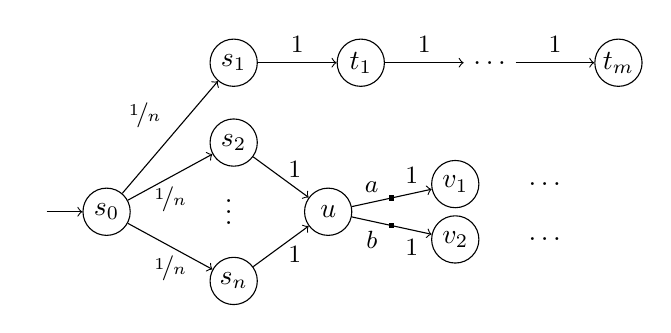
\begin{tikzpicture}
	\node[sstate, initial, initial text=] (s0) {$s_0$};
	\node[sstate,right=of s0, yshift=2.5em] (s2) {$s_2$};
	\node[sstate,above=0.4cm of s2] (s1) {$s_1$};
	
	\node[right=of s0,yshift=0.3em,xshift=0.2em] (sdots) {$\vdots$};
	\node[sstate,right=of s0, yshift=-2.5em] (sn) {$s_n$};
	\node[sstate,right=of s1] (t1) {$t_1$};
	\node[right=of t1] (tdots) {$\hdots$};
	\node[sstate,right=of tdots] (tn) {$t_m$};
	\node[sstate, right=2.2cm of s0] (u) {$u$};
	\node[sstate, right=of u, yshift=1em] (v1) {$v_1$};
	\node[sstate, right=of u, yshift=-1em] (v2) {$v_2$};
	\node[right=0.5cm of v1] {$\hdots$};
	\node[right=0.5cm of v2] {$\hdots$};
	
	
	
	\draw[->] (t1) -- node[elab] {$1$} (tdots);
	\draw[->] (tdots) -- node[elab] {$1$} (tn);
	
	\draw[->] (s0) -- node[elab] {$\nicefrac{1}{n}$} (s1);
	\draw[->] (s0) -- node[elab,below] {$\nicefrac{1}{n}$} (s2);
	\draw[->] (s0) -- node[elab,below] {$\nicefrac{1}{n}$} (sn);
	
	\draw[->] (s1) -- node[elab,above] {$1$} (t1);
	\draw[->] (s2) -- node[elab,near end,above] {$1$} (u);
	\draw[->] (sn) -- node[elab,near end,below] {$1$} (u);
	
	\draw[->] (u) -- node[actnode] {} node[elab,above, near start] {$a$}  node[elab,above, near end] {$1$} (v1);
	\draw[->] (u) -- node[actnode] {} node[elab,below, near start] {$b$} node[elab,below, near end] {$1$} (v2);
	
	
\end{tikzpicture}
\caption{}	
\end{figure}

\begin{example}
	Consider the SG (actually, an MDP) in Fig.~\ref{fig:drciOnSgs}. 
	First consider that under each scheduler, the path from $s_0$ to $t_m$ has probability $\nicefrac{1}{n}$. In particular, this means that a feasible DRCI instance (applied to an SG) must have $\ppthreshold \geq \nicefrac{1}{n}$. At the same time, every path in the SG already has probability at most $\nicefrac{1}{n}$, and thus, every schedulder that satisfies the randomness constraint for $\delta = 1$ satisfies it for any $\ppthreshold \geq \nicefrac{1}{n}$. Thus, DRCI does not allow us to enforce any kind of randomization in the $\pOne$-policy. 
\end{example}

On the other hand, for deterministic SGs, all randomization is due to the random behavior of $\pOne$. Roughly speaking, every path is then just good (i.e., ending in a target state) or bad (i.e., ending in a sink state). The randomization criterion then may just ensure that we do not select the same path with too much probability, which intuitively means that the $\pOne$-player must ensure in every step that there are a sufficient number of paths from the next state (no matter what $\pTwo$-player does). 
As long as there exist a sufficient number of paths, randomizing (uniformly) over those paths leads to a solution.

	For deterministic SGs, the set of feasbile ERCI and DRCI instances coincide.
\begin{theorem}
For any deterministic SG with some path sets $X_\varphi$, $X_\psi$ and threshold $\scthreshold$, 
there exists an $\pOne$-policy solving the DRCI problem with threshold $\ppthreshold$ iff there exists a $\pOne$-policy solving the ERCI problem with threshold $\randomness = f(\ppthreshold)$ for an adequate (computable) $f$.
\end{theorem}
We note that the policies solving the two problems do in general not coincide. 
\label{sec:related}
\color{red}
Maybe briefly discuss synthesis algorithms mentioned at start of intro?
\color{black}


\subsection{Additional Related Work}
 
Synthesis in MDPs with multiple hard and soft constraints (often over indefinite horizons) is a well-studied problem~\cite{DBLP:conf/stacs/ChatterjeeMH06,DBLP:conf/tacas/EtessamiKVY07,DBLP:conf/atva/ForejtKP12,DBLP:journals/fmsd/RandourRS17}.  In this setting, one generates deterministic policies and their convex combinations. Put differently, some degree of randomization is \emph{not an objective}, but rather a consequence. Interestingly, in \cite{DBLP:conf/tacas/DelgrangeKQR20} the optimal policies in \emph{absence} of randomization are investigated. Along similar lines, \cite{DBLP:journals/jcss/BrazdilCFK17} trades average performance for less variance, thereby implicitly trading off the average and the worst-case performance.  
The original results sparked interest in different extension to MDPs and the type of soft constraints, such as continuous MDPs \cite{DBLP:journals/csysl/HaesaertNS21} and continuous-time MDPs~\cite{DBLP:conf/cav/QuatmannJK17},  cost-bounded reachability \cite{DBLP:journals/jar/HartmannsJKQ20}, or mean-payoff properties~\cite{DBLP:journals/corr/abs-1104-3489}. 
The algorithms have also been extended towards stochastic games~\cite{DBLP:conf/mfcs/ChenFKSW13,DBLP:journals/sttt/KwiatkowskaPW18}.
Finally, notions of lexicographic multi-objective synthesis~\cite{DBLP:conf/cav/ChatterjeeKWW20} -- in which one optimizes a secondary criterion among all policies that are optimal with respect to a first criterion bare some resemblance with the algorithm we consider. 
These algorithms have been put in a robotics context in~\cite{DBLP:journals/ijrr/LacerdaFPH19}.
Finding policies that optimize reward objectives is well-studied in the field of reinforcement learning, and has been extended to generate Pareto-fronts for multiple objectives~\cite{DBLP:conf/icml/NatarajanT05,DBLP:conf/adprl/ParisiPSBR14}.

Randomization has been considered in different contexts. Entropy in MDPs is optimized in \cite{DBLP:journals/tac/SavasOCKT20}. 
\textcolor{red}{Marcell, do you have more on (causal) sentropy?}
Beyond Markov models, the (uniform) randomization over languages in finite automata \cite{DBLP:journals/siamcomp/HickeyC83,DBLP:conf/soda/KannanSM95} or over propositional formulae \cite{DBLP:journals/tcs/JerrumVV86,DBLP:journals/iandc/BellareGP00,DBLP:conf/dac/ChakrabortyMV14} has received quite some attention. Neither of those approaches support the notion of soft constraints or the related tradeoffs.

Path-finding has long been considered a multi-objective problem itself~\cite{DBLP:conf/icra/AmigoniG05,DBLP:journals/eswa/NazarahariKD19,DBLP:conf/icml/XuTMRSM20}.
These works differ prominently in two aspects: they do not trade-off randomization and performance, and they do not trade-off declarative and formal constraints with the accompanying formal guarentees, but are more search-based. 

Patrolling POIs and perimeters has received plenty of attention, e.g.,~\cite{DBLP:conf/icra/AgmonKK08,DBLP:conf/icra/AmigoniBG09,DBLP:conf/iros/PortugalPRC14}.  
Closest to our work are  formalisms rooted in game-theory,  such as  \emph{Stackelberg games}~\cite{simaan1973stackelberg,DBLP:conf/atal/ParuchuriPTOK07}. Stackelberg games have been extending to Stackelberg planning~\cite{DBLP:conf/aaai/SpeicherS00K18} in which a tradeoff between the cost for the defender and the attacker can be investigated.
Most related are the zero-sum~\emph{patrolling games} introduced in~\cite{DBLP:journals/ior/AlpernMP11}, which has led to numerous practical solutions~\cite{DBLP:books/daglib/0040483}. Patrolling games are explicitly games between an intruder and a defender, and there is no stochastic environment.  Adding additional objectives makes solving these problems harder~\cite{DBLP:conf/atal/Klaska0R20} and in general, the obtained policies are no longer applicable. To overcome this, a specific set of fixed objectives has been added to these games recently~\cite{DBLP:conf/atal/Klaska0R20}. 
 The large common aspect in all of this work is that optimal strategies do randomize. As in the synthesis work above, this is a consequence of the objectives rather than an objective in itself. 
 In comparison, we provide a general framework and in particular support stochastic environments.
 
%%% Local Variables:
%%% mode: latex
%%% TeX-master: "main"
%%% End:

\section{Conclusion}
This paper presented ERCI, a framework to control improvisation in stochastic games. Our results show that ERCI can be used to synthesize policies that besides meeting temporal logic specifications induce varying behavior, e.g., to test and certify the correctness of other robots. Future work includes applying the framework to a broader spectrum of applications and extending the theory to games with imperfect information.

{\vspace{0.5em} 
  \noindent\textbf{Acknowledgments}:
This work is partially supported by NSF grants 1545126 (VeHICaL), 1646208 and 1837132, by the DARPA contracts FA8750-18-C-0101 (Assured Autonomy) and FA8750-20-C-0156 (SDCPS), by Berkeley Deep Drive, and by Toyota under the iCyPhy center.}


\bibliographystyle{plainnat}
\bibliography{bibliography}


\section{Proofs}\label{sec:proofs}
\mypara{Convexity of ERCI solution set}
\begin{proof}[Proof Sketch Prop~\ref{prop:convex}]
  Recall that a set is convex, if it is closed under
  convex-combinations\footnotemark. Consider two points
  $\langle \scp, \rndp \rangle, \langle \scp', \rndp' \rangle \in
  \solutions$ achieved by $\pOneSched$ and $\pOneSchedPrime$
  respectively. Consider the new policy, $\pi$, defined by employing
  $\pOneSched$ with probability $q$ and $\pOneSchedPrime$ with
  probability $\bar{q} \eqdef 1 - q$.  Because each policy
  \emph{guarantees} its corresponding performance, this new policy as
  performance at least $q\cdot \scp + \bar{q}\cdot \scp'$.  Similarly,
  by viewing $\pi$ as a random variable and applying chain rule
  yields,
  \begin{equation}
    \begin{split}
      H_\tau(\sigma)
      \geq &~q \cdot H( \rv{A}^{\pOne}_{1:\tau'} \mid\mid \rv{S}_{1:\tau} \mid \pi=\pOneSched)~+\\
      &~\bar{q}  \cdot H( \rv{A}^{\pOne}_{1:\tau'} \mid\mid \rv{S}_{1:\tau} \mid \pi=\pOneSchedPrime)\\
      =&~q\cdot\rndp + \bar{q}\cdot \rndp'.
    \end{split}
  \end{equation}
  Thus, any convex combination of guaranteed points is guaranteed by
  a convex combination of the corresponding ego policies.
\end{proof}


\subsection{Completeness of Entropy Matching for SGs}


\begin{proof}[Proof Sketch of SG Completeness]
  First, observe that on games with only sink nodes, completeness
  follows directly.  Next, suppose the entropy matching family is
  complete on all sub-graphs of $\sg$. To simplify our proof, observe
  that w.o.l.o.g., we can restrict our attention to ERCI instances
  on the Pareto front, $\langle \scthreshold,\randomness\rangle \in \pareto{\solutions}$.
  Next, for the sake of contradiction, we shall assume that no entropy
  matching policy achieves $\langle \scthreshold,\randomness\rangle$,
  but $\sched_{\pOne}^*$ does:
  \begin{align}
    &\forall \sched_\pOne \in \{\sched^{\pOne}_\rat\}_\rat~.~ x_{\sched_{\pOne}} \prec \langle \scthreshold, \randomness \rangle\label{eq:reject}\\
    &\exists \sched_\pOne^* \notin \{\sched^{\pOne}_\rat\}_\rat~.~  \langle \scthreshold, \randomness \rangle \preceq x_{\sched_{\pOne}^*}\label{eq:incomplete}.
  \end{align}
  Note that because the entropy matching family contains the maximizers and minimizers
  of entropy, and because increasing rationality monotonically decreases entropy,
  there must exist some rationality, $\rat$, such that $\sched_\pOne^\rat$ has:
  \begin{equation}
    \rndp_{\sched_\pOne^\rat} = \randomness = \rndp_{\sched_\pOne^*},
  \end{equation}
  where the second equality follows from the ERCI instance being on the Pareto front.
  Next, let $\sched_\pTwo^\rat$ denote the min-randomness
  $\pTwo$-policy given $\sched_\pOne^{\rat}$. Because $\sched_\pOne^*$
  witnesses $\langle\scthreshold, \randomness\rangle$, it must be the case
  that:
  \begin{equation}\label{eq:pareto_bound_for_rat}
    \rndp_{\langle \sched_\pOne^*, \sched_\pTwo^\rat \rangle} \geq \randomness
    \hspace{3em} \wedge \hspace{3em}
    \scp_{\langle \sched_\pOne^*, \sched_\pTwo^\rat\rangle} \geq \scthreshold
  \end{equation}
  However, because $\sched_\rat$ indexes the Pareto front for MDPs,
  one must be tight. Further, because of uniqueness of MaxEnt policies
  for non-trivial ERCI instances in MDPs, one equality
  in~\eqref{eq:pareto_bound_for_rat}, implies both are tight! Thus,
  \begin{equation}
    \begin{split}
      &\rndp_{\langle \sched_\pOne^\rat \sched_\pTwo^\rat \rangle} = \randomness = \rndp_{\langle \sched_\pOne^*, \sched_\pTwo^\rat \rangle}\\
      &\scp_{\langle \sched_\pOne^\rat \sched_\pTwo^\rat\rangle} = \scthreshold = \scp_{\langle \sched_\pOne^*, \sched_\pTwo^\rat\rangle}  
    \end{split}
  \end{equation}
  Thus, due to uniqueness of MaxEnt MDPs $\sched_\pOne^\rat$ and
  $\sched_\pOne^*$ must exactly match on $\sg[\sched_\pTwo^\rat]$ and
  must differ on some other subgraph.  Applying the inductive
  hypothesis, we know that the entropy matching family is complete on
  these subgraphs, and thus if $\sched_\pOne^*$ achieves a given
  $\langle\scthreshold, \randomness\rangle$ on this sub graph, there
  must be an entropy matching that does so as well.  However, by an
  exchange argument, this implies that:
  \begin{equation}
    x_{\sched_{\pOne}^*} \preceq x_{\sched_{\rat^*}},
  \end{equation}
  contradicting
  assumptions~\eqref{eq:reject} and \eqref{eq:incomplete}.  Thus,
  entropy matching must be complete.
\end{proof}

\mypara{ERCI and RCI coincide}
\begin{proof}[Proof Sketch of Prop~\ref{prop:conservative}]

  First, observe that as in ERCI, for RCI, one can w.o.l.g. assume
  $\pTwoSched$ is deterministic~\cite{DBLP:conf/cav/FremontS18}.
  Thus, given some worst-case adversary (for randomness and
  performance) all randomization is due to the behavior of
  $\pOne$. Assuming a non-trivial solution set (and thus
  $\scopt \neq 0$), this implies that $\pOne$ can \emph{first} decide
  whether to meet the soft constraint and \emph{then} choose actions
  weighted by the number of guaranteed ways to reach $\target$ in the
  corresponding subtree. Now observe when planning against the
  min-causal entropy adversary, $\sched_*^\pTwo$, the deterministic SG
  reduces to a deterministic MDP. In deterministic MDPs, the action
  sequence uniquely determines the state sequence, and thus the causal
  entropy reduces to the entropy of the actions and states, i.e., the
  paths, $\xi$.  Thus, treating $\xi$ as a random variable and
  case splitting on winning yields:
  \begin{equation}\label{eq:cond_win}
    \begin{split}
      h_{\langle \sched_\pOne, \sched^*_\pTwo\rangle} &= \scthreshold\cdot H(\xi \mid \text{win}) + (1 - \scthreshold)\cdot H(\xi \mid \neg \text{win})\\
      &\leq \scthreshold\cdot \log(\#\text{win}) + (1 - \scthreshold)\cdot \log(\#\neg
      \text{win})
    \end{split},
  \end{equation}
  where $\#\text{win}$ and $\#\neg \text{win}$ are the
  number of paths to $\target$ and $\sink$ respectively and equality holds
  for the policy that selects paths uniformly. Furthermore, notice that this policy
  bounds the maximum probability of a trace given the performance:
  \begin{equation}
    \ppthreshold \geq \max\left(\frac{\scthreshold}{\#\text{win}}, \frac{ 1- \scthreshold}{\#\neg \text{win}}\right).
  \end{equation}
  It follows then that the inverse of the Pareto characteristic
  function determines the causal entropy threshold needed to decide the RCI instance
  using RCI, i.e.,
  \begin{equation}
    \begin{split}
      \randomness &= \rndmin + \rndopt\cdot (\delta - \rndmin)\\
      &= \rndmin + \rndopt \cdot \Big (\solfuncp^{-1}\left(\frac{\scthreshold - \scmin}{\scopt}\right) - \rndmin\Big)
    \end{split}.
  \end{equation}
\end{proof}

Thus, one can view ERCI as a conservative extension of RCI to stochastic games.

%%% Local Variables:
%%% mode: latex
%%% TeX-master: "main"
%%% End:


\end{document}

%%% Local Variables:
%%% mode: latex
%%% TeX-master: t
%%% End:

